\documentclass[a4paper,11pt]{article}
\usepackage[utf8]{inputenc}
\usepackage[T1]{fontenc}
\usepackage{amsmath,amssymb}
\usepackage{mathtools}
\usepackage{algorithm}
\usepackage{algorithmicx}
\usepackage{algpseudocode}
\usepackage{float}
\usepackage{xcolor}
\usepackage{url}
\documentclass{article}
\usepackage{graphicx}
\usepackage{tikz}
\usepackage{siunitx}

\begin{document}

\section{Introduction}
Generally speaking, an ABM is a computational model in which one defines the behaviour of a single or different kinds of agents and makes them interact via a rule-based framework. Therefore, each agent is defined both in space and time trought a set of mutable and/or fixed attributes. In ABM, there are three main steps to accomplish: define an agent, determine agents' behaviours and implement the interactions. With their bottom-up approach, these models find large applications in ecology, social sciences, economics, studies of traffic jams etc. \cite{ABM}. In addition to their capability of obtaining outcomes similar to the empirical ones, another advantage of ABMs in the context of DeFi is that they can be used to simulate a market environment similar to the real one on which different policy can be tested.

\section{Uniswap Agent Based Model}
The general idea is to take the ABM developed by Angeris et al. \cite{angeris2021analysisuniswapmarkets} and extend it in the context on Uniswap v3’s concentrated liquidity. The presence of a liquidity profile different from a uniform one (as in the case of Uniswap v2), changes how the price moves in response to a trade and how Liquidity Providers (LPs) choose the price range during the mint operations.

I think it should be sensible to construct three models of increasing complexity:

\begin{enumerate}
    \item Angeris’ model in Uni v3. The agents will be just Arbitrageurs, LPs and Traders. Trading is done in continuous time (no mempool, no block time).
    \item Angeris’s model in Uni v3 with the presence of a memory pool. The agents are again Arbitrageurs, LPs and Traders. They post their order in the mempool and after the block time is passed, everything is executed at once (i.e. discrete trading on the DEX). During the block time, the CEX price evolves.
    \item Final ABM with the presence of the MEV searcher that exploit their power in the mempool by performing back running arbitrages, sandwich attacks and JIT liquidity provision (see MEV section for reference)
\end{enumerate}
Within each model, I can consider sub models with and without gas fees and/or slippage tolerance. The important changes to implement are related on how swaps and mint events are handeled in the concentrated liquidity framework. Specifically, the former are performed iteratively tick by tick, while the latter are governed by different dynamics with respect to Uniswap v2.

\subsection{Motivation}
The goal of the project is to devise an ABM model of Uniswap with concentrated liquidity in order to use it as a generative machine of realistic market dynamics under different conditions on volatility and/or liquidity. Quite recently, Uniswap introduced the forth version of his AMM, Uniswap v4. At the core, it has the same trading mechanisms as the previous version, with a constant product rule and concentrated liquidity. The key innovation has been the introduction of the so-called \textit{hooks} that can be thought as additional smart contracts that sits on top of the pool's one. These hooks give the possibility of greater customization of the behaviour of a pool. For instance, one can implement a dynamic fee mechanisms that respond to specific market conditions. Specifically, the goal is to use it to answer the following question:
\begin{itemize}
    \item What kind of dynamic fee mechanisms (that can be introduced in the newer Uniswap v4, that has the same skeleton as v3 but with the possibility of adding the so-called \textit{hooks}, i.e. additional smart contract that sits on top of the pool's one) provide stable revenues for liquidity providers?
\end{itemize}
% \subsection{How I want to implement the model}
% Currently I am not an expert on what I going to say here, but I learned that I can fork the Ethereum mainnet and let my agents talk to the real Uniswap V3 pools in order to bypass any deployment from scratch. This will allow me to use the built in functions of Uniswap that handle swaps, mints and burns efficiently.

\subsection{Recap of swap math in Uniswap v3}
In Uniswap the price is always indicated as the ratio between the token1 reserves and the token0 reserves (hence, token0 is the numéraire). In what follows, token0 $\to A$ and token1 $\to B$. Additionally, I will not include the fee rate $\tau$ in the following expressions. It would only scale the actual swapped amount by $r=(1-\tau)$.

Remember that Uniswap v3 stores only the liquidity $L$ and the square root price $S=\sqrt{P}$. When performing a swap, two situations can occur:

\subsubsection{Single tick swap} 
In this case Uniswap v3 acts like Uniswap v2. The liquidity $L$ is constant and only $S$ changes.

\begin{itemize}
    \item \textbf{Swap $\Delta_a \to \Delta_b$ }
    \begin{equation}
        S_{target}= \frac{L S_t}{L + \Delta_aS_t}, \qquad \Delta_b = L(S_t -S_{target})
    \label{1}
    \end{equation}
    \item \textbf{Swap $\Delta_b \to \Delta_a$ }
    \begin{equation}
        S_{target} = S_t + \frac{\Delta_b}{L}, \qquad \Delta_a = L\left(\frac{1}{S_t}-\frac{1}{S_{target}}\right)
        \label{2}
    \end{equation}
\end{itemize}

\subsubsection{Tick Crossing}
In this case the swap is the iteration of single tick swaps until there is no remaining quantity to trade. Specifically, at the beginning of the swap Uniswap evaluates the next square root price of the next tick boundary (the one toward which $S$ is moving), $S_{tick}$

\begin{itemize}
    \item \textbf{Swap $\Delta_a \to \Delta_b$ }
    Uniswap evaluates the amounts $\Delta_{a}^{tick}$ needed to reach $S_{tick}$ as (from \ref{1})
    \begin{equation}
        \Delta_{a}^{tick} = \frac{L(S_{tick}-S_t)}{{S_{tick}S_t}}
    \end{equation}
    If $\Delta_{a}^{tick} > \Delta_a$, a single tick swap is performed and the procedure is stopped. Otherwise the current tick will output an amount 
    \begin{equation}
        \Delta_{b}^{tick} = L (S_t-S_{tick})
    \end{equation}
    The remaining quantity $\Delta_{a}^{rem} = \Delta_a-\Delta_a^{tick}$ is swapped in the next tick by repeating the process with the next $S_{tick}$ and $L$, until $\Delta_{a}^{rem}=0$
    \item \textbf{Swap $\Delta_b \to \Delta_a$ }
    The reasoning is the same but we need to use slightly different formulas.
    Again, given $S_{tick}$ as the square root price of the next tick boundary, firstly assess the amount $\Delta_b$ needed to reach it (from \ref{2})
    \begin{equation}
        \Delta_b^{tick} = L(S_{tick} - S_t)
    \end{equation}
    If $\Delta_{b}^{tick} > \Delta_b$, perform a single tick swap and stop. Otherwise, you will have as output of the current tick swap
    \begin{equation}
        \Delta_{a}^{tick}=L\left(\frac{1}{S_t}-\frac{1}{S_{tick}}\right)
    \end{equation}
    The remaining quantity $\Delta_{b}^{rem} = \Delta_b-\Delta_b^{tick}$ is swapped in the next tick by repeating the process with the next $S_{tick}$ and $L$, until $\Delta_{b}^{rem}=0$
\end{itemize}

\section{Reference market}
In Angeris’ model, there are two price dynamics: one for a reference market (CEX), denoted $m^p_t$, and one for the Uniswap market, denoted as $S^2_t$. From now on, $m^p_t$ will refers to the price of token A with respect to token B.

 $m^p_t$ moves according to a permanent impact generated by trading a quantity $\Delta_a$ of token A for a quantity $\Delta_b$ of token B

 \begin{equation}
     m^p_t \to m^p_t + \kappa \text{sign}(\Delta_a) |\Delta_a|^{1+\xi}
 \end{equation}

 and, after this effect has been incorporated, by a diffusion process

 \begin{equation}
     m^p_t \to m^p_t e^{\sigma X+\mu} \qquad X \sim N(0,1)
 \end{equation}

\section{Mempool}
The mempool can be thought of as a waiting room where orders are appended before they are validated. In DEXs, the presence of the mempool significantly changes the way trades are executed. Indeed, the submission transaction order is not equal to the execution transaction order due to the presence of specialized agents, the MEV searchers, that rearrange, add, and/or remove, orders from the mempool to gain a personal profit. Furthermore, the trades on the DEX cannot be performed continuously, but actually must wait a certain amount of time before executed (block-time). 

To implement the mempool in the model, the idea is to divide each simulation step into multiple sub-periods in which the agents submit the orders into the mempool. Even if the AMM is not updated until the block-time has passed, the reference market moves every time an arbitrageur adds an order to the mempool. This is due to the fact that CEX-DEX arbitrages are non-atomic. Then, after the block-time, all the orders are executed at once on the DEX and its state is updated.

\section{Agents}
\subsection{Arbitrageurs}
I will keep the no arbitrage condition derived in Angeris with an additional condition on liquidity. Indeed, you need also enough cumulative liquidity along the swap path to push the price up/down to the arbitrage band.

Let:
\begin{itemize}
  \item $S_\star = \sqrt{r m_p}$ the no-arbitrage target price in the token1 $\to$ token0 direction,
  \item $S^\star = \sqrt{r^{-1} m_p}$ the no-arbitrage target in the token0 $\to$ token1 direction,
  \item $L(S)$ the piecewise-constant liquidity function defined over ticks,
  \item $S_{\max}$ the upper bound of the last populated tick (for increasing $S$),
  \item $S_{\min}$ the lower bound of the first populated tick (for decreasing $S$).
\end{itemize}

\begin{equation}
\boxed{
\begin{aligned}
&\text{If } S^2_0 < r\,m_p:\quad
  \int_{S_t}^{S_\star} \! L(S)\,S^{-2} \, dS
  \;\le\;
  \int_{S_t}^{S_{\max}} \! L(S)\,S^{-2} \, dS, \\[10pt]
&\text{If } S^2_0 > r^{-1} m_p:\quad
  \int_{S^\star}^{S_t} \! L(S)\, dS
  \;\le\;
  \int_{S_{\min}}^{S_t} \! L(S)\, dS.
\end{aligned}
}
\end{equation}

\textbf{Interpretation:}
\begin{itemize}
  \item The arbitrageur \emph{would} push the price to the fee-adjusted external price ($r m_p$ or $r^{-1} m_p$),
  \item but he can do so \emph{only if} the pool offers enough cumulative liquidity along the path to support the necessary volume.
  \item If liquidity runs out before reaching $\sqrt{r m_t^p}$ or $\sqrt{r^{-1} m_t^p}$, arbitrage terminates early and the price remains outside the no-arbitrage band.
\end{itemize}

In the following, I will indicate with a superscript the market from which the quantity is obtained (it is not strictly required, but it can help follow the reasoning) and with $C_{A\to B}(\cdot)$ and $C_{B\to A}(\cdot)$ the Uniswap functions that dictate the output of a swap. Specifically

\begin{align}
C_{A\to B}(r\Delta_a) &= L(S_t -S_{target})
\nonumber
\\ 
C_{B\to A}(r\Delta_b) &= L\left(\frac{1}{S_t}-\frac{1}{S_{target}}\right)
\nonumber
\end{align}

Assuming an infinitely liquid reference market, there are two possible scenarios:   
\begin{enumerate}
    \item $S^2_t \geq {r^{-1}}m^p_t$ : Uniswap is more expensive than the reference market.
    
    The arbitrageur takes a loaned amount $\Delta_{b}$ of tokens B and buys $\Delta_a^{CEX}=\frac{\Delta_{b}}{m^p_t}$ of tokens A on the reference market. Then, he goes on Uniswap and swaps the $\Delta_a^{CEX}$ tokens A for $\Delta_{b}^{UNI} = C_{A\to B}(\Delta_a^{CEX}) = C_{A\to B}(r \frac{\Delta_{b}}{m^p_t})$, generating a profit of $\Delta_{b}^{UNI}-\Delta_b = C_{A\to B}(r \frac{\Delta_{b}}{m^p_t})-\Delta_b$

    \item $S^2_t \leq r m^p_t$ : Uniswap is cheaper than the reference market.
    
    The arbitrageur takes a loaned amount $\Delta_{b}$ of tokens B and buys $\Delta_a^{UNI} = C_{B\to A}(r\Delta_b)$ of tokens A on Uniswap. Then, he goes on the reference market and sells the $\Delta_a^{UNI}$ tokens A for $\Delta_{b}^{CEX}=m^p_t\Delta_{a}^{UNI}=m^p_t C_{B\to A}(r\Delta_b)$, generating a profit of $\Delta_{b}^{CEX}-\Delta_b = m^p_t C_{B\to A}(r\Delta_b)-\Delta_b$
\end{enumerate}
Therefore, an arbitrageur seeks to maximize the difference $\Delta_{a}^{'} - \Delta_a$ where $\Delta_a^{'}$ is either $C_{B\to A}(r \frac{\Delta_{a}}{m^p_t})$ or $m^p_tC_{A\to B}(r\Delta_a)$ depending on the direction of the arbitrage.

\subsection{Liquidity Providers}
In Uniswap v3 a liquidity provider must choose both the amount to mint and the provision range. In Angeris LPs choose how to act according to a Markowitz optimization problem. Here, I think it can be better to use something inspired by the optimal provision strategy derived in Monga’s PhD Thesis \cite{monga2024automatedmarketmakingdecentralized} or the reasoning in Capponi et al. \cite{capponi2021liquidity}.  The general finding is that LPs tend to widen their provision range as the volatility of the exchange rate increases. This is due, as explained in Capponi, to the risk of adverse selection. For instance, we can make the liquidity providers choose a symmetric range around the current price $P_t$ according to the EWMA of the discrepancy between CEX and DEX price in the last $\tau$ steps.

Let $B_t$ measures how much the price is beyond the no arbitrage band

\begin{equation}
    B_t = \max{\left(0, |\log S_t^2 - \log m_t| - \log \left(\frac{1}{r}\right)\right)}
\end{equation}

Now construct the EWMA of $B_t$

\begin{equation}
    D_t = \lambda D_{t-1} + (1-\lambda)B_t \qquad \lambda=e^{-\ln(2)/h}
\end{equation}

where $h$ is the half-life in number of steps.

The half width is then evaluated as

\begin{equation}
    w_t = w_{min} + \psi \frac{D_t}{\log(1.0001)} + |\epsilon_t| \qquad \epsilon_t=Y_t-np, \quad Y \sim Bin(n,p)
\end{equation}


% \begin{equation}
%     w_t=w_{min} +\psi \frac{V_\tau^{arb}}{V_\tau^{tot}} + |\epsilon_t|, \qquad \epsilon_t=Y_t - np, \quad Y \sim Bin(n,p)
% \end{equation}
where $w_{min}$ is the half of the minimum tick range allowed that depends on the fee tier of the pool and $\psi$ is a scale parameter that controls how the provision range reacts to the discrepancy between CEX and DEX prices. $\epsilon_t$ is a noise contribution that introduces heterogeneity. It follows a binomial distribution with parameter $(n,p)$, centered around zero. Finally, we clip the total width of the LP position to the nearest multiple of the tickSpacing parameter, since in Uniswap v3 only those positions can be created.

% NOTE: Empirically, over 1 year (2023) of data of the USDC-WETH 0.05\% pool, 46\% of all the mints and burns corresponds to the minimum tick range allowed (10). There is also a 0.5\% cases in which the LP mint in the entire possible range (I suppose it is the max 1774540.0). This value is a significant spike with respect to the previous ones that, after values of $\sim 2000$ for the tick range, are almost 0\%.

This expression also incorporates the effect of high volatility. 
% In high volatilty regimes, the volume swapped by the arbitrageurs ( $V^{arb}_t$) increases, since there will be more probability of a bigger gap between the reference market price and the Uniswap price. 

At the beginning, the liquidity profile is composed by a certain number of liquidity providers' positions that form a binomial distribution centered at the initial price $S^2_0$. In total, There are $N$ liquidity providers (LPs), categorized as either active or passive. Active LPs adhere to the profit-and-loss (PnL) rule (described below) and also re-center their minted positions whenever the price remains outside their range for $k_{\text{out}}$ consecutive steps. Passive LPs, by contrast, follow only the PnL rule. The initial liquidity is added by a set of active LPs. Then, $\forall t > 0$, a LP will draw a liquidity value $l=\frac{2L_0}{N}X$ with $X\sim|N(0.01,0.02)|$ and $L_0$ being the active liquidity at time zero (the initial binomial distribution), and choose to mint it with a certain probability (higher for the active LP) in a symmetric price range of width $w_t$ around the current  price $S^2_t$.

Every LP stores all their opened positions details: quantities minted, price range, fee accrued up to the current time, impermanent loss at the current time. They decide to burn a position whenever the profits made by fee collection minus the impermanent loss exceed a certain take profit threshold or when hit a stop loss threshold.

The impermanent loss at time $t$ is the difference between the value of an LP's position (comprising token A and token B) in a Uniswap pool at time $t$, $ \mathcal{P}^{\text{LP}}_t$, and the value of a portfolio holding the original amounts of token A and token B (as minted initially), each valued at their current reference market prices, $\mathcal{P}^{\text{HODL}}_t$ 

\begin{equation}
    \text{IL}_t = \mathcal{P}^{\text{LP}}_t - \mathcal{P}^{\text{HODL}}_t \leq 0
\end{equation}
Then, if $F_t$ is the value of the total fee collected up to time $t$, the Profit and Loss of an LP is

\begin{equation}
    \text{PnL} = F_t + \text{IL}_t
\end{equation}

Finally, he decides to burn his position when either

\begin{equation}
    \text{PnL} \geq \theta_{TP} \quad \text{or} \quad \text{PnL} \leq -\theta_{SL}
\end{equation}
 with $\theta_{TP}, \theta_{SL} >0$ are the take profit and stop loss thresholds.
\subsection{Traders}
I would keep these kind of agents as in Angeris’ work. That is, a trader will perform a swap in a certain direction on Uniswap as long as the cost of trading on Uniswap does not exceed the cost of trading the same amount on the reference market by some constant percentage $\theta_{Tr}$. Specifically, the trader will draw the quantity $\Delta_a$ (or $\Delta_b$) from some probability distribution and check if performing this trade in the Uniswap market is at most some percentage more expensive than performing it in the reference market. If not, he executes the trades, otherwise he will not.

$\forall t>0$, a trader will draw a Bernoulli variable to choose the swap direction and an amount $\Delta_{a,b}$ from a certain probability distribution and choose to trade it on Uniswap if the trade will output an amount $ m_t^p\Delta_{a,b} \leq (1+\theta_{Tr})C(r\Delta_{a,b})S^2_t $.

The probability distribution from which the trader samples the amount to swap is set to be a normal distribution in the log amount. In other words, the trader sample an amount $\Delta_{a,b} \sim \exp{N(\mu, \sigma)}$. Actually, the empirical log amount swapped is well described by a  mixture of gaussians, but we will keep it simple and use just one normal distribution (even because the mixture probably stems from other strategic traders, not the noisy ones).

\section{Simulations}
\subsection{ABM 1: continuous trading, no MEV, random actor orders}

\begin{algorithm}[H]
\caption{First sketch of ABM for Uniswap v3}\label{alg:abmv3}
\begin{algorithmic}[1]
  \Require Total steps $T$, model parameters
  \State Initialize reference price $m^p_0$, Uniswap price $S^2_0$ and liquidity distribution.
  \State Initialize populations of Traders, Arbitrageurs and LPs. An LP can be passive or active.
  \For{$t = 1$ to $T$}
  \State \textbf{Randomize sequence of actors and split the LPs in 3 groups that act around the trader and arbitrageur} \smallskip
  \State \textbf{Traders submit swaps}
    \ForAll{Trader}
      \State Draw direction $d\in\{A\!\to\!B,B\!\to\!A\}$ and size~$\Delta$
      \If{$m_t^p\Delta \leq C(r\Delta)(1+\theta_{Tr})$}
        \State \Call{Swap}{$d,\Delta$}
        \State Update liquidity profile and $S^2_t$
      \EndIf
    \EndFor
    \smallskip

    \State \textbf{Arbitrageurs exploit gaps}
    \ForAll{Arbitrageur}
      \If{$S^2_t \ge r^{-1}m^p_t$}
        \State Compute optimal $\Delta a^*$. Buy on CEX and sell on Uniswap
        \State Update liquidity profile and $S^2_t$
      \ElsIf{$S^2_t \le r\,m^p_t$}
        \State Compute optimal $\Delta a^*$. Buy on Uniswap and sell on CEX
        \State Update liquidity profile and $S^2_t$
      \EndIf
    \EndFor
    \smallskip


    \State \textbf{Liquidity Providers adjust}
    \ForAll{LP}
      \State Compute range width 
        $w_t \gets  w_{min} + \psi \frac{D_t}{\log(1.0001)} + |\epsilon_t|$
      \State Draw new liquidity $l=\frac{2L_0}{N}X$ with $X\sim|N(0.01,0.02)|$
      \If{rand()$<$mintProb}
        \State Mint $L^\mathrm{new}$ in $[\sqrt S^2_t-w_t,\sqrt S^2_t+w_t]$
      \EndIf
      \State Update fees $F_t$, impermanent loss $\text{IL}_t$, PnL
      \If{PnL $\ge \theta_{TP}$ \textbf{or} PnL $\le -\theta_{SL}$}
        \State Burn position
      \EndIf
    \EndFor
    \smallskip

    \State \textbf{Update reference market price}
    \State $\Delta_T = \Delta a + \Delta$
    \State Trade impact
      $\Delta m^p_t \gets \kappa\,\mathrm{sign}(\Delta_T)\,|\Delta_T|^{1+\xi}$
    \State $m^p_t \gets m^p_{t-1} + \Delta m^p_t$, then diffuse
      $m^p_t \gets m^p_t\exp(\sigma X + \mu)$
    \smallskip

    % \State \textbf{6. Log all metrics}
  \EndFor
\end{algorithmic}
\nonumber
\end{algorithm}



This is the simplest specification. We create an ABM for Uniswap v3 where the trading is continuous in time in both the CEX and the DEX. Therefore, there is no mempool and no special ordering of the actions on the DEX. For each step, we randomize the sequence of the actors, keeping the update of the CEX price at the end of each step.


Not all the LPs act together: each one has a clock that ticks on average every $\tau$ steps (sampled from a geometric distribution). Only when the clock ticks they are active. Additionally, we divide the active LPs in 3 groups and spread them around the abritrager and the trader (group 1 -> trader -> group 2 -> arb -> group 3). This has been implemented to reduce the herding effects that clusterized heavily the activity.


Even if the realism of this model is far from satisfying, we can already notice one big difference from the Uniswap v2 like ABM of Angeris or Di Fazio: due to the presence of concentrated liquidity, the DEX price does not stay always in the no arbitrage bands. Sometimes, the arbitrage does not have sufficient liquidity to push the price to its profit-maximizing level, i.e. the nearest boundary of the band.

% TODO: talk about OFAC regulated relayes (mevwatch.info)
\section{Maximal Extractable Value}
\label{sec:mev}

It is worth making a digression about how the orders are submitted and validated on the Ethereum blockchain. Indeed, the peculiar framework employed allows the agents charged with handling orders to extract profit from transaction manipulations through operations like rearrangements, additions, or removals. These profits add on top of the standard rewards and transaction fees. In general, this kind of gain is known as Maximal Extractable Value (MEV)\footnote{Historically, it has been introduced as Miner Extractable Value, see \cite{daian2019flash}.}, and it is one of the core dynamics present in DEXs and, so, in Uniswap v3. \\

\subsection{Proposer-Builder Separation (PBS)}
In TradFi, orders are processed instantaneously, and the time difference between submission from the user and insertion in the limit order book is usually of the order of milliseconds. Therefore, it is quite impossible to find trades sharing the same exact timestamp. On the other hand, the order flow in DEXs is lumpy, as transactions are grouped into blocks that are validated sparsely in time, currently, on the Ethereum blockchain, every 12 seconds. This means that the orders submitted are not immediately active in the market, but instead need to wait before being added to the blockchain. The orders submitted between the validation of two blocks are received by an Ethereum node and stored in the so-called memory pool (\textit{mempool}). We can think of the mempool as a 'waiting room' where transactions stay before being validated and appended to the next block. The (public) mempool is the best field in which MEV proliferates. At a high level, the mechanism of MEV extraction is quite simple: since all the information about the pending transaction is accessible to everyone\footnote{For example, via Ethernow \url{https://ethernow.xyz/mempool/all}}, in the period between the validation of two adjacent blocks, all users have the possibility to add their own transaction to the mempool and exploit the effects of what the currently pending transactions will have (that can be simulated deterministically). Before 2022, traders fighting for MEV, that we will call from now on \textit{MEV searchers}, kept offering higher and higher priority fees \footnote{The priority fee is a tip that the users add to their transacations to gain prioriy in the mempool. It is one of the two components of the transactions fees (knwon as gas fees). The other one is the base fee, chosen deterministically based on the previous blocks congestion. It is burned, so no one gain it.}so that the miner or validator would place their transaction first. Ordinary users got caught in the cross-fire and had to pay much higher fees for any kind of operation, especially during events prone to high MEV rents. For example, an MEV searcher that wants to front run a large swap, should have attached to the front run swap an higher priority fees than the victim swap to rank before it.

Around 2022, in the Ethereum community a new concept started to be discussed \cite{buterinPBS2021}: the Proposer-Builder-Separation (PBS), a mechanism aimed to distribute the role of creating new blocks among different actors with the aim of reducing centralization, censorship and the negative effects of the priority gas fee wars just described \footnote{technically, they are called Priority-Gas Auctions (PGAs)}. PBS changes who constructs a block by separating the builder role (execution + ordering) from the proposer role (consensus). The validator still runs the execution engine to verify the final payload before signing. The former is put in the hand of the \textit{block builders}, the latter operated by the \textit{proposer}, i.e. the validators. Currently, PBS is implemented by third party services, and so it is not an active part of the consensus protocol on Ethereum, but the Ethereum research and client development communities are working towards a protocol-level implementation of PBS, which is expected to be included in a future hard fork \cite{ethereumPBS2024}.

The most adopted software implementation of the PBS is MEV-Boost by Flashbots (\url{https://boost.flashbots.net/}). Almost 90\% of the blocks are currently validated using MEV-Boost \cite{mevboost_pics}. Again, the general idea is to distribute the role of creating block to a new actor, the \textit{block builder}, and delegate just the validation of the block to the validator. The block builder receives (atomic \footnote{An atomic transaction is either fully executed or totally reverted, depeding wehther its actions are feasible.}) bundles of transactions constructed by the MEV searchers from the mempool in a bid-auction mechanism. The searchers therefore must attach a bribe to the bundles and the auction is handled off-chain. Then, builders construct block proposals that are submitted to a validator, again in a bid-auction mechanism which is managed by trusted third-parties known as \textit{relays}. Relays act as neutral brokers: builders stream just the block headers plus bids to the relays, the validator asks each relay for its best header and signs the richest one . Finally the relay reveals the full block only after it sees the validator’s signature that guarantee a fair exchange between the two parties, preventing the validator from stealing the builder’s work and the builder to under-bid the validator. Figure \ref{fig:pbs_schema} illustrates this chain of actions. For a more detailed description of this chain of actors, see \cite{oz2024wins}. Therefore, huge gas-fee spikes are now less common because the bidding happens off-chain, between builders, not in the public mempool, see Figure \ref{fig:historical_gasprice}. On the other hand, even if one of the goals was to reduce the centralized power that validators had, PBS moved this power to an even smaller set of professional builders that handle most blocks, so the system is more orderly but also more centralized than before. Figure \ref{fig:builder_relay_validator}, taken from \cite{mevboost_pics}, shows the flows of the block proposal from the block builders to the validators, through the relays. Additionally, there is also the risk of a relay failure, as already happened \cite{marzecThibault2024} \cite{damatoNeuder2023}.

\begin{figure}
    \centering
    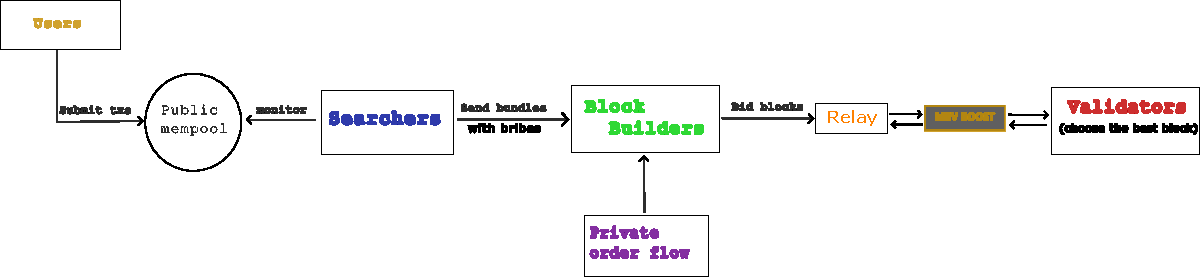
\includegraphics[width=0.8\linewidth]{figures_st_app/pbs.pdf}
    \caption{PBS schema}
    \label{fig:pbs_schema}
\end{figure}
However, this is not the entire story, as in the last couple of years high-value wallets and bots have increasingly bypassed the public mempool, sending bundles straight to builders via 'private RPC' channels. This exclusive order flow (EOF) gives the builder a first (often sole) look at the trade, letting them avoid public priority gas fee auctions, pair the transaction with an optimal back-run \footnote{Usually, there are agreements between the order flow provider and the block builder that allows the latter to just front run the former}, and quote a bigger bid to the validator, increasing the chance of winning the next block.
Depending on the agreement, part of the extracted MEV may be rebated to the EOF sender, or the sender may pay a flat coin-base tip for protection against MEV. 

Summarizing, we have three main actors in PBS: MEV-searchers, Block Builders and Validators. Their profits can be written as

\begin{figure}
    \centering
    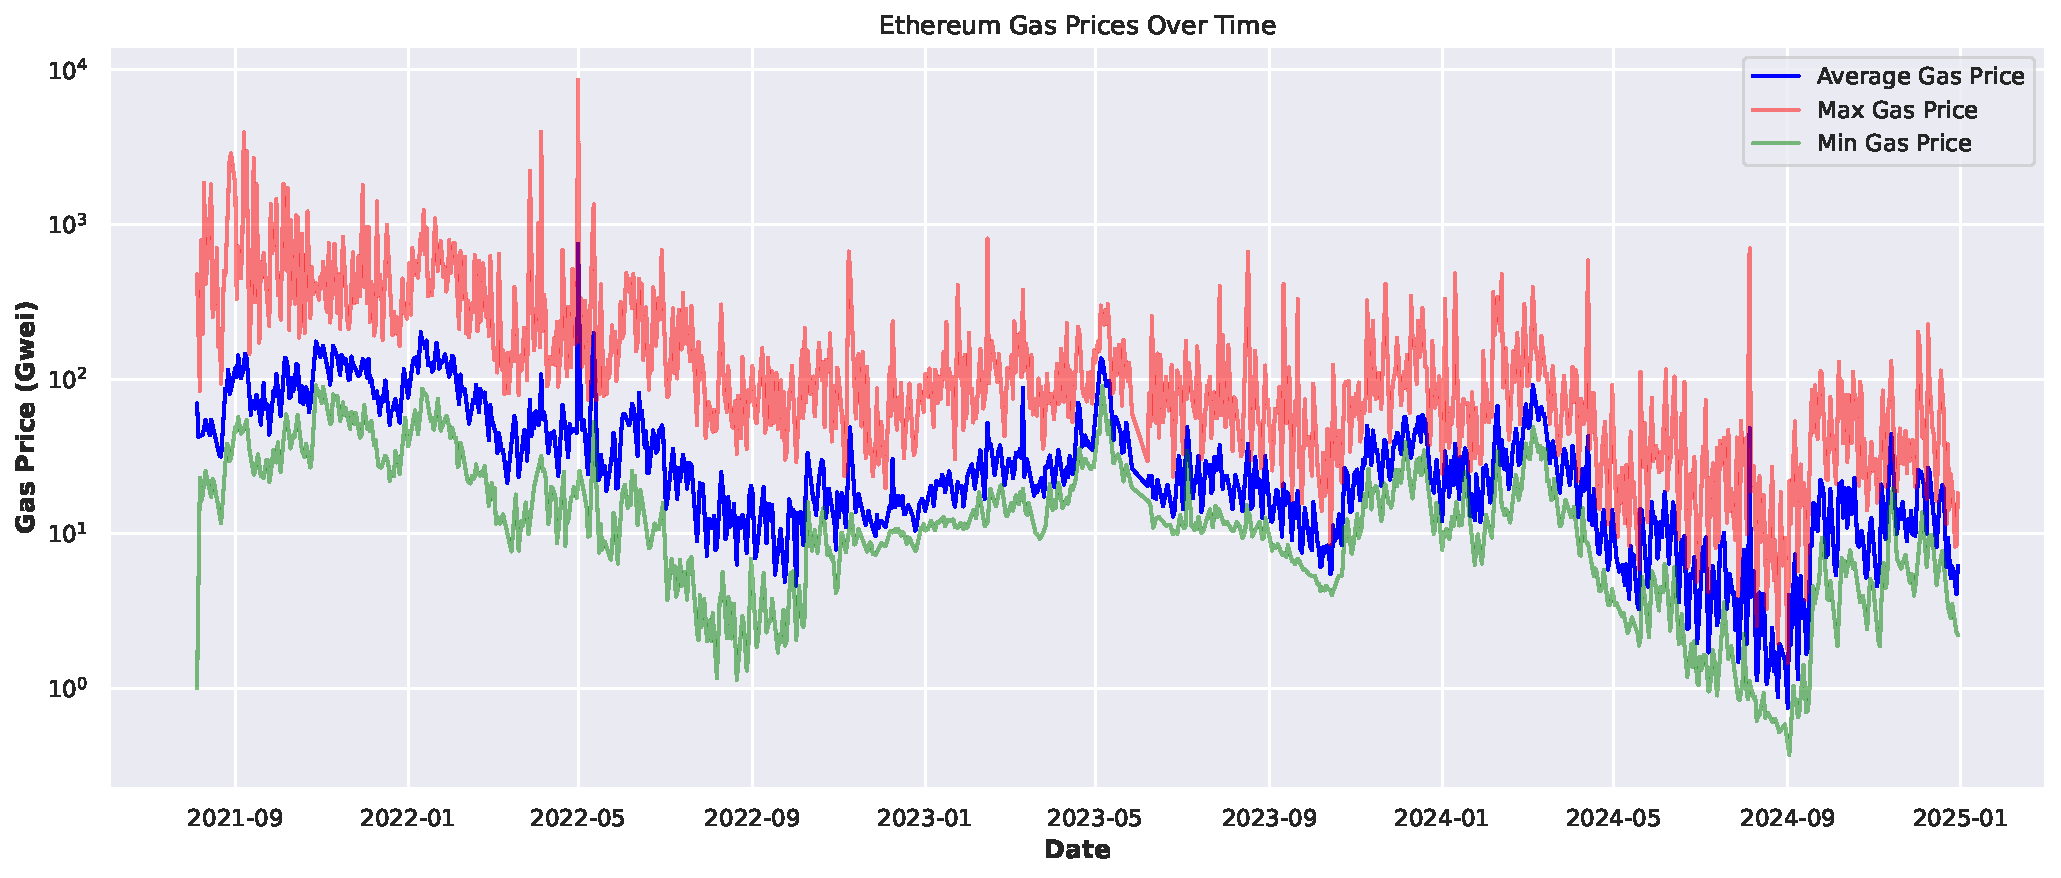
\includegraphics[width=0.8\linewidth]{figures_st_app/historical_gas_prices.pdf}
    \caption{Hiastorical gas price from 05/08/2021 (first available day of the DexGuru Ethereum Gas Tracker) to 31/12/2024. The Min Gas Price represents the lowest fee paid for a transaction to be included in a block, while the Max Gas Price is the highest fee paid in that same block — reflecting the range of urgency and cost users were willing to pay. }
    \label{fig:historical_gasprice}
\end{figure}
\vspace{1em}

%-----------------------------------------------------------------------
% 2 Profit functions
%-----------------------------------------------------------------------
%----------------------------------------------------------
% Profit functions (ETH units, per block)
%----------------------------------------------------------
\begin{align}
\textbf{Searcher:}\quad
\pi_s &= M
        -\bigl(
            C_{\text{gas}}
          + D_{\text{sb}}
          + C_{s,\text{infra}}
        \bigr) \\[6pt]
%
\textbf{Builder:}\quad
\pi_b &= R
        - \bigl(1+\rho\bigr)B   % bid paid to validator plus relay fee
        - R_{\text{refund}}     % on-chain user rebate
        - C_{b,\text{infra}} \\[6pt]
%
\textbf{Validator:}\quad
\pi_v &= B
        + R_{\text{consensus}}
        - C_{v,\text{infra}}
\end{align}

%----------------------------------------------------------
% Refund calculus (inside the same block)
%----------------------------------------------------------
\[
   R_{\text{refund}}
      \;=\; \varphi\,D_{\text{sb}},\qquad
   0\le \varphi \le 1.
\]

%----------------------------------------------------------
% Raw block value (unchanged from the papers)
%----------------------------------------------------------
\[
  R = \sum_{i\in\text{tx}}
        \bigl(
          \text{priority fee}_i
          + \text{direct transfer}_i
        \bigr).
\]

%----------------------------------------------------------
% Symbol glossary (additions in blue)
%----------------------------------------------------------
\begin{center}
\begin{tabular}{@{}ll@{}}
\toprule
Symbol & Meaning \\ \midrule
$R$ & Raw block value (priority-fee tips $+$ direct transfers) \\
$B$ & Builder\,$\to$\,proposer payment (coinbase transfer) \\
$M$ & MEV revenue realised in the searcher’s bundle(s) \\
$C_{\text{gas}}$ & Gas actually paid by the searcher’s bundle \\
$D_{\text{sb}}$ & Direct ETH transfer (tip) from searcher to builder \\
$\varphi$ & Refund ratio ($0\!-\!1$) set by MEV-Share or similar \\
$R_{\text{refund}}$ & On-chain rebate to user: $\varphi D_{\text{sb}}$ \\
$\rho$ & Relay-fee fraction on the builder’s bid ($0\!-\!1$) \\
$C_{s,\text{infra}}$ & Off-chain infrastructure costs of the searcher \\
$C_{b,\text{infra}}$ & Builder infrastructure \& order-flow costs \\
$C_{v,\text{infra}}$ & Validator infrastructure costs \\
$R_{\text{consensus}}$ & Protocol-level block-proposal reward \\ \bottomrule
\end{tabular}
\end{center}


% where $\text{refund}_b$ is the portion of the value a bundle generates that is explicitly routed back to the original order-flow owner (the user, wallet, or dApp that sent the protected transaction).
% It only appears when the bundle travels through an Order-Flow Auction (OFA) such as Flashbots Protect / MEV-Share or MEV-Blocker.
% In those channels the user agrees to share enough data about their transaction to let searchers back-run it, but on the condition that they receive a preset share of whatever MEV is realised
% \[
% \begin{aligned}
% \Pi_{\text{searcher}}
% &=
% \sum_{b \in \text{bundles}}
% \Bigl(
% \underbrace{\Delta\mathrm{state}_{b}}_{\substack{\text{value extracted}\\\text{by the searcher}}}
% \;-\;
% \underbrace{\mathrm{gas}_{b}}_{\substack{\text{gas fees}\\\text{paid on-chain}}}
% \;-\;
% \underbrace{\mathrm{bribe}_{b}}_{\substack{\text{priority-fees or}\\\text{coinbase tips to builder}}}
% \;-\;
% \underbrace{\mathrm{refund}_{b}}_{\substack{\text{any rebate or}\\\text{OFA refund paid}}}
% \Bigr)
% \\[1em]
% \Pi_{\text{builder}}
% &=
% \underbrace{v_{\text{true}}}_{\substack{\displaystyle\sum_{i}\bigl(\mathrm{tip}_{i}+\mathrm{cb}_{i}-\mathrm{refund}_{i}\bigr)\\\text{(total block value)}}}
% \;-\;
% \underbrace{(1+\rho)\,\mathrm{bid}}_{\substack{\text{payment to proposer}\\\text{plus relay fee}}}
% \\[1em]
% \Pi_{\text{validator}}
% &=
% \underbrace{\mathrm{bid}}_{\text{builder→proposer payment}}
% \;+\;
% \underbrace{\gamma\sum_{i}\mathrm{tip}_{i}}_{\substack{\text{priority fees}\\\text{from each tx}}}
% \;+\;
% \underbrace{\mathrm{issuance}}_{\substack{\text{staking rewards}\\\text{(new ETH minted)}}}
% \;-\;
% \underbrace{\mathrm{penalties}}_{\substack{\text{slash fines or}\\\text{missed duties}}}
% \end{aligned}
% \]
\begin{figure}
    \centering
    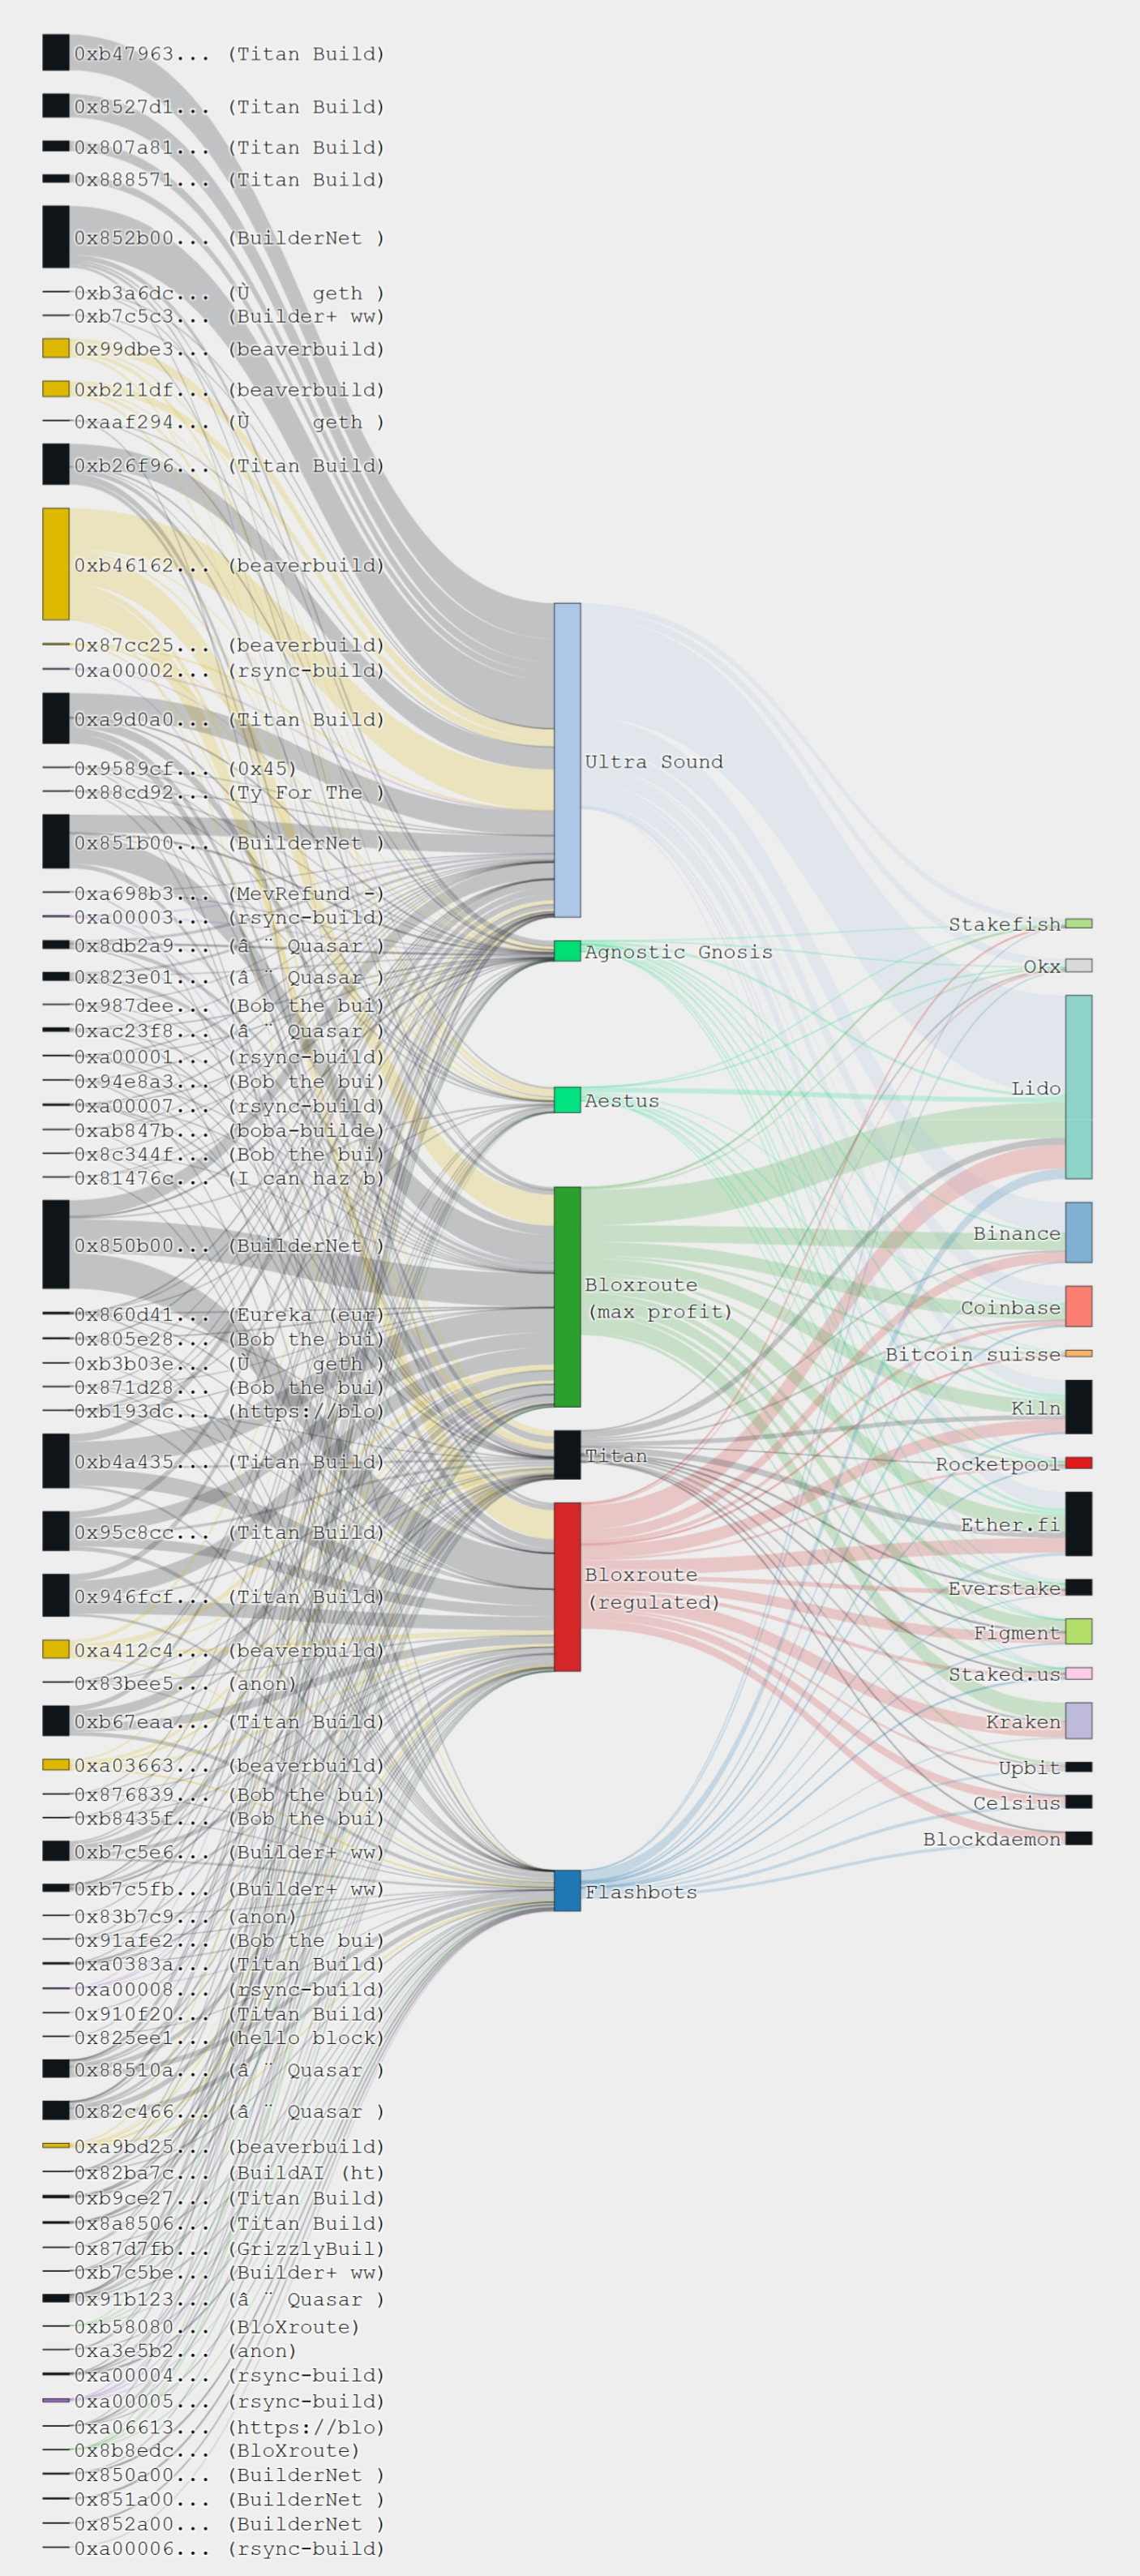
\includegraphics[width=0.5\linewidth]{figures_st_app/blockbuilder_relay_validator.png}
    \caption{Caption}
    \label{fig:builder_relay_validator}
\end{figure}
\subsection{MEV Strategies}
In this section we present  a narrative that walks through different MEV strategies and carefully draws parallels to its closest equivalent in traditional finance (TradFi), unpacking how each tactic works, what the motivations are, and where the two domains differ due to rules, infrastructure, or ethics. 
We will focus on the most widely used strategies \footnote{For a comprehensive survey about MEV in DeFi, see \cite{materwala2024maximal}.}. They include arbitrages, sandwich attacks and Just-in-Time liquidity. 

\subsubsection{Flash--loan attacks}
\label{subsec:flashloans}

A flash loan allows any Ethereum user to borrow  an arbitrary amount of ERC-20 liquidity without any kind of collateral provided that the entire borrow $\rightarrow$ exploit $\rightarrow$ repay sequence is executed atomically inside a single transaction.  This means that the lender’s solvency risk is zero (the call reverts if the repayment fails). All the strategies described below can (and actually do) include a flash loan as initial step. Indeed, a meta-study of the 100 largest DeFi hacks through 2024 finds that roughly
60\% of all price-manipulation exploits relied on flash loans
\cite{halborn2024survey}. In addition, flash loans can also be used to perform hijack on governance-tokens based protocols, like Decentralized Autonomous Organizations (DAOs). In this case, the attacker flash-borrow $>$51\,\% of a token supply, pass a malicious proposal in the same transaction, drain the treasury, and repay.

There is no analogue of unlimited, unsecured and atomic credit in TradFi.

\subsubsection{Arbitrage}
In these cases, MEV searchers can exploit price mismatches between two pools, two DEXs or even DEX and CEX. In such a way, they contribute to market efficiency. We can distinguish between atomic arbitrages and non-atomic arbitrages. The first ones involve only on-chain operations and are executed using atomic transactions to buy the cheaper asset and simultaneously sell the more expensive one, usually within a single block. Furthermore, thanks to the atomicity of smart contracts, the searcher can also take advantage of flash loans \footnote{A flash loan on Ethereum is a type of unsecured loan offered by certain decentralized finance (DeFi) protocols (e.g., Aave or dYdX) that allows users to borrow assets instantly and without collateral, as long as the loan is repaid within the same blockchain transaction} to perform the strategy without upfront capital. It is therefore an almost riskless strategy since if the transaction fails, the searcher only loses the gas fee paid. Instead, non-atomic arbitrages refer to DEX-CEX arbitrages, where the searcher must interact with an off-chain platform (the CEX) and so she cannot exploit the atomicity of the smart contracts, exposing herself to the risk of a non-profitable arbitrage due to adverse price movements before the validation of her transactions.

What we have just described can be labeled as beneficial for the market, since it helps the information flows trough the different market venues in the DeFi ecosystem. However, it is important to note that there are some malicious types of arbitrage that can be called 'price manipulation arbitrages'. In this scenario, a user takes a flash loan, uses part of it to borrow a token (like WBTC) on a lending platform, and another part to execute a leveraged trade that pushes up the token’s price on a low-liquidity AMM. They then sell the borrowed tokens at the inflated price and repay the flash loan, keeping the profit. All of this is possible due to smart contract bugs being exploited.

In order to understand this dynamics, it can be helpful to illustrate one famous example of this attack. It happened in 2020 on the protocol bZx. In that case, the attacker did exactly what we have already discussed: he took a flash loan of 10,000 ETH and used 5,500 ETH as collateral on Compound to borrow 112 WBTC, while using 1,300 ETH to open a 5x leveraged margin trade on bZx. The margin trade routed through Kyber and executed a large ETH-to-WBTC swap on Uniswap, which had low liquidity at the time. This trade itself caused the price of WBTC to spike from around 38 ETH to over 109 ETH. Due to a bug in the bZx smart contract, the system failed to perform a proper collateralization check after the trade and accepted the manipulated price as valid. As a result, the attacker was able to sell the 112 borrowed WBTC for 6,871 ETH, repay the 10,000 ETH flash loan, and walk away with a net profit of around 1,271 ETH, worth approximately \$355,000 at the time, leaving the protocol with bad debt.

In traditional finance, this maps closely to multi-venue arbitrage, a classic strategy in equity and FX markets. High-frequency trading (HFT) firms monitor multiple exchanges using direct, ultra-low-latency data feeds. When they detect a stale price on one venue they race to buy low and sell high before the prices converge. Similar strategies are used between ETFs and their underlying baskets.

Key differences:
\begin{itemize}
    \item In TradFi, trades are not atomic—there’s real execution and inventory risk during the latency window.
    % \item Under MiFID II’s best-execution mandate—enforced in Italy by CONSOB—brokers must seek the best possible result across Borsa Italiana, MTFs and systematic internalisers, effectively delivering an NBBO-like outcome for Italian investors.
    \item in TradFi infrastructure is a huge barrier: collocation, proprietary data feeds, and microwave networks can cost tens of millions annually.
    \item In DeFi, a simple Ethereum transaction with the right logic can do the same work for a few dollars in gas.
\end{itemize}

% \subsubsection{Liquidations}
% DeFi lending protocols like Aave or MakerDAO allow anyone to liquidate under-collateralized positions by repaying part of the borrower’s debt and receiving a discounted portion of their collateral. This happens automatically as soon as the loan-to-value (LTV) ratio breaches a set threshold, and liquidators (MEV searcher) compete openly to be the first to act.

% In TradFi, this parallels margin calls and default liquidations in brokerage and derivatives markets. When an investor’s equity drops below the maintenance margin, their broker issues a margin call. If not met within a specific timeframe, the broker forcibly liquidates their position—usually via smart-order routing that seeks best execution. In futures markets, clearinghouses like CME organize default auctions where member firms bid to take over the risk of failing counterparties. Repo markets do similar things via General Collateral Finance (GCF) auctions.

% Key differences:
% \begin{itemize}
%     \item TradFi liquidations are centrally managed by brokers or clearinghouses, with best-execution obligations and reporting duties (e.g., Form 1099-B in the U.S.).
%     \item DeFi liquidations are decentralized and public: any address can try, and speed is determined by gas and mempool positioning.
%     \item TradFi gives borrowers time to cure margin violations. DeFi executes the liquidation in the very same block that LTV fails.
% \end{itemize}

\subsubsection{Sandwich attacks}
Sandwich attacks are strategies designed for gaining from the price impact of a large swap (performed by the victim) pending in the mempool. The MEV searcher acts as follows. Firstly, a swap is placed in the same direction as the victim (also known as front run); then, the victim swap is executed \footnote{There is of course the possibility of multiple victims' swaps}; lastly, the attacker closes the position by placing a swap with the same amount and opposite sign to the front run (also known as back run). This type of attack harms market participants, as the victim pays a higher price due to the impact of the front run swap.

The victim can protect herself from this type of attack by setting a low slippage tolerance on her transaction. This means that if the swap would result in receiving less than a certain minimum amount, the transaction will automatically fail. As a result, the attacker must carefully choose how much to front-run—if they push the price too far, the victim’s transaction will not go through, and the attack fails.

The TradFi analogue is front-running, either in its classic form (e.g., a broker trading ahead of a client order) or in more modern, legal gray zones like latency arbitrage. HFT firms use predictive models and "ping" orders to infer large institutional activity. If detected early, HFTs may quickly buy shares in one venue before the order hits and sell them at a slightly higher price moments later.

Key differences:
\begin{itemize}
    \item On Italian markets, dealing on non-public client information is prohibited by the EU Market Abuse Regulation (MAR) and Articles 184-187-ter of Italy’s Consolidated Finance Act (TUF), so front-running is a criminal behaviour.
    \item In DeFi, the mempool is public. This makes sandwich attacks legally murky: technically, the bot is acting on public data, not insider information.
    \item TradFi has surveillance systems, anti-internalization rules, and dark pool disclosures. DeFi is experimenting with privacy-preserving alternatives (e.g., encrypted mempools, SUAVE) but lacks formal enforcement.
\end{itemize}

\subsubsection{Just-in-Time (JIT) liquidity}
JIT liquidity is a strategy for gaining the fee that a large swap in the mempool will pay once executed. The MEV searcher deposits liquidity in a very narrow price range (containing the current price) just before the transaction is processed, earning most of the trading fee, and removes the liquidity immediately after the transaction. This strategy is also referred to as \textit{LP sandwich} or \textit{active liquidity provision}\footnote{Despite this definition is very appealing, it should not be confused with the so-called \textit{active liquidity}, that is the sum of all the liquidity whose range contains the price.} \cite{capponi2023paradox}, as the liquidity provision is elicited by a pending order in the mempool. The liquidity provider never intends to provide ongoing liquidity; they simply "ride" the trade. In contrast to sandwich attacks, JIT liquidity is beneficial for the end user due to the enhanced liquidity that lower the price impact of the swap.

In TradFi there is not a direct analogue of this strategy, but it resembles fleeting quotes and rebate-seeking behavior. On venues available to Italian firms, HFTs sometimes flash tight quotes on pan-European MTFs such as Cboe Europe CXE/BXE, which still rebate about 0.15 bps to passive fills. By contrast the main Euronext Milan order book merely waives or halves the passive fee rather than paying cash.
% Market makers also internalize retail flow only when conditions are favorable—like in payment-for-order-flow (PFOF) systems where brokers route trades to wholesalers who offer price improvement and liquidity only when profitable.

Key differences:
\begin{itemize}
    \item TradFi exchanges now limit these tactics. MiFID II empowers CONSOB and Borsa Italiana to impose order-to-trade-ratio caps and minimum quote-life parameters, preventing excessive 'quote flicker' by HFT algorithms.
    \item In Uniswap, there is no time-in-force constraint—adding and removing liquidity can happen in a single atomic transaction.
    \item TradFi rebates are paid by the venue; in DeFi, traders themselves pay LP fees. The design incentive is inverted.
\end{itemize}



\subsubsection{Mixed (Sandwich+JIT) attacks}
It is worth noting that the state-of-the-art to exploit a large swap in DeFi is a combination of JIT and Sandwich attacks. When a large swap is detected in the mempool, a mixing attack made up of a JIT encapsulated into a sandwich could sometimes bring the highest profit. Specifically, the exact scheme is: front run, mint liquidity, victim swap, burn liquidity, back run.\\


\noindent MEV strategies aren’t new—they are just smart-contract-powered expressions of long-standing financial instincts: arbitrage, front-running, fleeting liquidity provisioning etc. What sets DeFi apart is its:
\begin{itemize}
    \item \textbf{Atomicity}: execution is all-or-nothing in a single block
    \item \textbf{Transparency}: everything is visible (and exploitable) in the mempool.
    \item \textbf{Permissionlessness}: anyone with code and gas can participate—no licenses, no seat fees.
\end{itemize}

Meanwhile, TradFi imposes structural constraints through surveillance, regulatory rules, and operational friction (e.g., latency, risk desks). But at their core, both systems reward the same thing: speed, insight, and the ability to act before others do. 

\section{Which strategy?}
The main choice that an MEV searcher is faced to understand what is the best strategy to employ according to the size of the victim's swap. In this section, we derive the profits of four different strategies:
\begin{enumerate}
    \item Just-in-Time (JIT) liquidity
    \item Back run arbitrage
    \item Sandwich Attack
    \item Mixed strategy JIT+Sandwich Attack
\end{enumerate}
These profits, minus the gas fees paid to perform them, correspond to the maximum bribe that the MEV searcher can pay to the block builder while guaranteeing a positive profit.
Table \ref{tab:notation} summarizes the notation used in this section

Throughout this section we adopt the standard Uniswap v3 single-tick equivalence: let $S=\sqrt{P}=\sqrt{Y/X}$ be the square-root price and $L$ the active liquidity. Define the virtual reserves $\tilde{x}=L/S$  and $\tilde{y}=LS$. Within a tick, swaps update $(\tilde{x},\tilde{y})$ exactly as a constant-product AMM, and an ultra-narrow JIT mint is a liquidity bump $L\mapsto(1+\alpha)L$ that keeps the price fixed. All formulas in this section hold if  $x_i,y_i$ are interpreted as $\tilde{x}_i,\tilde{y}_i$ and no tick boundary is crossed during anu leg (front-run, victim, burn, back-run). A tick-aware generalization rule (multi-tick traversal with updates to $L$) is provided in Appendix A.

The analysis values every term in token $X$ using the pre‑strategy marginal price $P_0 = y_0/x_0$.

We use the term "victim" to refer to the user whose swap is included in the bundle. However, this label can be misleading in certain contexts. In JIT liquidity provision, the strategy often benefits the user by reducing price impact through enhanced liquidity. Similarly, in back-run arbitrage, the user's transaction remains unaffected, as the arbitrage occurs after their swap and does not inflict any harm.

\begin{table}[H]
\centering
\begin{tabular}{ll}
\hline
\textbf{Symbol} & \textbf{Meaning} \\
\hline
$f$ & Uniswap fee rate (e.g., 0.0005, 0.003, 0.01) \\ \hline
$S$ & Size of the victim's swap (in token $X$) \\ \hline
$\sigma$ & Normalized victim's swap size, $S = \sigma x_0$ \\ \hline
$r$ & Net input rate after fee, $r = 1 - f$ \\ \hline
$s$ & Attacker front-run input (in token $X$) \\ \hline
$\varepsilon$ & Normalized front-run size, $s = \varepsilon x_0$ \\ \hline
$\alpha$ & Multiplier of the reserves chosen by the searcher for LP \\ \hline
$x_0, y_0$ & Pool reserves before the beginning of the strategy \\ \hline
$P_0$ & Marginal-price of $X$ in terms of $Y$ before before the beginning of the strategy, $P_0 = y_0/x_0$ \\ \hline
$I$ & Price impact \\ \hline
% $v$ & Net amount of token $X$ added by the victim, $v = r S$ \\ \hline
$\Delta y_{\text{fr}}$ & Token $Y$ output from the front-run \\ \hline
$\Delta y_{\text{br}}$ & Token $Y$ input in the back-run \\ \hline
$\Delta x_{\text{br}}$ & Token $X$ output from the back-run \\ \hline
% $S_{\text{br}}$ & Size of the back-running swap in token $X$, $S_{\text{br}} = r S$ \\ \hline
$G_{\text{JIT}}$ & Gas cost of mint + burn operations for JIT \\ \hline
$G_{\text{br}}$ & Gas cost of back-running swap \\ \hline
$G_{\text{sand}}$ & Total gas paid by the sandwich attacker \\ \hline
$m_{\text{JIT}}$ & Bribe or validator payment in JIT \\ \hline
$m_{\text{br}}$ & Bribe or validator payment in back-run strategy \\ \hline
$m_{\text{sand}}$ & Bribe or validator payment in sandwich attack \\ \hline
\end{tabular}
\caption{Unified notation for MEV strategy modeling.}
\label{tab:notation}
\end{table}



\subsection{JIT profits}
A JIT liquidity provider (LP) monitors the public Ethereum mempool and spots a pending swap of size $S$ from $X$ to $Y$. The LP constructs a single-bundle transaction with the following operations:

\paragraph{Mint.} Just before the victim swap, the MEV searcher provides liquidity in an ultra-narrow tick range (typically, the smallest possible one dictated by the pool parameter \textit{tickSpacing}). If the current tokens' reserves are $x_0, y_0$, she provides $\alpha x_0$ and $\alpha y_0$, with $\alpha > 0$. Hence,  she owes a fraction $\frac{\alpha}{\alpha+1}$ of the range.
The reserves are now

\begin{equation}
    (x_0,y_0) \mapsto (x_1,y_1) = \left(x_0(1+\alpha), y_0(1+\alpha)\right)
\end{equation}
\paragraph{Victim swap(s) (X$\to$Y).} The victim swaps $S=x_0\sigma$ tokens X for $\Delta y_v$ tokens Y such that
\begin{equation}
    x_1y_1 = (x_1+rS)(y_1-\Delta y_v) \implies\Delta y_v = \frac{y_0(1+\alpha) r \sigma}{1+\alpha+r\sigma}
\end{equation}
Therefore the reserves become
\begin{equation}
    (x_1,y_1) \mapsto(x_2,y_2) = \left(x_0(1+\alpha+r\sigma), \frac{y_0 (1+\alpha)^2}{1+\alpha+r\sigma}\right)
\end{equation}
\paragraph{Burn.} Now, the MEV searcher removes her liquidity, burning a fraction $\frac{\alpha}{\alpha+1}$ of the new reserves $(x_2, y_2)$.

\begin{align}
    \Delta x_{burn} &= \frac{\alpha}{1+\alpha}x_0(1+\alpha+r\sigma) \\
    \Delta y_{burn} &= \frac{\alpha}{1+\alpha}\frac{y_0(1+\alpha)^2}{1+\alpha+r\sigma}
\end{align}

The difference between the burn amount and the mint amount is
\begin{align}
    \Delta x_{burn} - \alpha x_0 &= \frac{\alpha}{\alpha+1}x_0r\sigma \\
    \Delta y_{burn} - \alpha y_0 &= - \frac{\alpha y_0 r \sigma}{1+\alpha+r\sigma}
\end{align}

We will omit, for the moment, the hedging costs that the JIT LP faces when providing liquidity. Indeed, she takes the other part of the trade with respect to the victim, exposing herself to the token. Ideally, she would open an opposite position on another venue (usually, a CEX) to cover it \footnote{Therefore, the profit equation must be seen as an upper bound.}. Therefore,
the LP's expected profit is bounded above by
\begin{align}
    \Pi_{\text{JIT}} &=   \underbrace{\frac{\alpha}{\alpha +1}\sigma x_0f}_{\text{fee earned}}{} + \underbrace{\frac{\alpha}{\alpha+1}x_0r\sigma}_{\text{LP change in token X}} - \underbrace{\frac{\alpha y_0 r \sigma}{1+\alpha+r\sigma}\frac{x_0}{y_0}}_{\text{LP change in token Y valued at }P_0} \\
    &=\frac{\alpha}{\alpha +1} x_0 \sigma - \frac{\alpha r \sigma}{1+\alpha+r\sigma}x_0
\end{align}
% \begin{equation}
% \Pi_{\text{JIT}} = Lf  - G_{\text{JIT}} - m_{\text{JIT}}.
% \end{equation}
% Non‑negative profit therefore requires that the bribe the searcher is willing to pay to the block builder is such that
% \begin{equation}
% m_{\text{JIT}} \le Lf  -  G_{\text{JIT}}\label{eq:max_jit_bid}
% \end{equation}
% In what follows we assume that the JIT LP is able to collect fees on the entire victim's swap \footnote{In case of a partial harvest, just add a multiplicative factor $\lambda \in [0,1]$}. This means that
% \begin{equation}
% \boxed {m_{\text{JIT}} \le Sf  -  G_{\text{JIT}}\label{eq:max_jit_bid}}
% \end{equation}
\subsection{Back-running arbitrage option}
%---------------------------------------------------------------
The simplest alternative to JIT is to just arbitrage the price impact generated by the user transaction. A classic MEV back-runner would take a flash loan \footnote{We assume that the cost of the flash loan is zero.} and lets the victim’s swap push the pool price. Then she would trade in the opposite direction to harvest the transient spread.

In this case, the bundle is composed by just two operations

\paragraph{Victim's swap}
The victim swaps $S$ tokens $X$ in the pool (direction $X\to Y$).
After the victim leg the reserves become
\begin{equation}
    (x_0,y_0) \mapsto (x_1,y_1)=( x_0 + rS, y_0 - \Delta y_v)
\end{equation}
where
\begin{equation}
\Delta y_v
  =y_0\,\frac{r\sigma}{1+r\sigma}.
\end{equation}
If $P_0$ is the initial price and $P_1$ are, respectively, the initial and final prices in terms of the X token, the price impact $I$ induced by this swap is

\begin{equation}
    I = \frac{P_1}{P_0} - 1 = \frac{1}{(1 + r\sigma)^2} - 1
\label{victim_impact}
\end{equation}
\paragraph{ Back‑run arbitrage trade}
The arbitrageur must choose the optimal amount $\Delta y_{br}$ to trade in the opposite direction (swap $Y\to X$) to maximize her profits $\Pi_{br}$. In general the profit function can be written as the difference between what she obtain from the arbitrage swap, indicated with $\Delta x_{br}$, and what she has paid. Therefore, evaluating everything in token X, we have
\begin{equation}
    \Pi_{br} = \Delta x_{br} - \frac{\Delta y_{br}}{P_0}
    \label{eq:arbitrage_profit}
\end{equation}

where $P_0$ is the initial price. Now we have to workout the value of $\Delta x_{br}$ as a function of $\Delta y_{br}$. This can be simply obtained from the constant product rule

\begin{equation}
    (x_1 - \Delta x_{br}) (y_1 + r \Delta y_{br}) = x_1y_1 \implies \Delta x_{br} = \frac{x_1 r \Delta y_{br}}{y_1 + r\Delta y_{br}}
\end{equation}
Using \eqref{eq:arbitrage_profit}, we obtain

\begin{equation}
    \Pi_{br} = \frac{x_1 r \Delta y_{br}}{y_1 + r\Delta y_{br}} - \frac{\Delta y_{br}}{P_0}
    \label{eq:arbitrage_profit1}
\end{equation}

Setting the derivative of $\Pi_{br}$ to zero and solving for $\Delta y_{br}$, we obtain that the optimal back-run size is

\begin{equation}
    \Delta y_{br}^* = \frac{y_0}{r}\left[\sqrt{ r} - \frac{1}{1+r\sigma}\right]
\end{equation}
that is greater than zero when
\begin{equation}
    \sigma \geq \frac{1/\sqrt{r} -1}{r}  \simeq \frac{f}{2}
\end{equation}
Or, equivalently, when $|I|>f$. 

The price after the optimal trade is
\begin{equation}
    P_2 = \frac{y_2}{x_2} = r P_0
\end{equation}
The arbitrageur trades until the final price equals the start price after deducting the fee; therefore, a positive fee always leaves an un-reverted spread. In the case of zero fee, the price is totally reverted, bringing back the reserves to their initial state.
Plugging $\Delta y_{br}^\star$ into \eqref{eq:arbitrage_profit1} we obtain the maximum profit achievable
\begin{equation}
\Pi^*_{br}(\sigma) = x_0
\frac{ \left(\sqrt{r}(1+r\sigma)-1\right)^2}{r(1+r\sigma)}
\end{equation}
%---------------------------------------------------------------
% \paragraph{Backrunning arbitrage vs JIT}

% We now reconsider the comparison between a back-running arbitrage and a JIT liquidity strategy, incorporating the optimal arbitrage strategy derived earlier.
% \\

% \noindent Including the gas cost $G_{\text{br}}$, the backrun strategy has a bribe ceiling:
% \begin{equation}
% m_{\text{br}}^{\max} = \Pi_{\text{br}}^{\star} - G_{\text{br}}.
% \end{equation}
% Instead, remember that JIT liquidity provider can offer up to
% \begin{equation}
% m_{\text{JIT}}^{\max} = Sf - G_{\text{JIT}}.
% \end{equation}
% Let $\varphi = \frac{G_{\text{JIT}} - G_{\text{br}}}{S}$ denote the gas differential per victim token. Setting $m_{\text{br}}^{\max} = m_{\text{JIT}}^{\max}$ leads to:
% \begin{equation}
% \Pi_{\text{br}}^{\star} = S(f - \varphi).
% \end{equation}
% that is
% \begin{equation}
% \frac{ \bigl(\sqrt{r} (1+r\sigma) - 1\bigr)^2}{r(1+r\sigma)}\;=\sigma\bigl(f-\varphi\bigr).
% \label{eq:equality_raw}
% \end{equation}

% Let  $u = 1 + r\sigma$ and $g=f - \phi$. From \eqref{eq:equality_raw} we get

% \begin{equation}
% (r-g)u^2  + (g - 2\sqrt{r}) u + 1 = 0
% \end{equation}
% whose positive root is
% \begin{equation}
%     u^* = \frac{2\sqrt{r} -g + \sqrt{(g-2\sqrt{r})^2} - 4(r-g)}{2(r-g)} \implies \sigma^* = \frac{u^*-1}{r}
% \end{equation}

% The builder will include the JIT bundle whenever its bribe ceiling
% exceeds that of the optimal back-run, i.e.  
% whenever the left‐hand side of \eqref{eq:equality_raw}
% is \emph{smaller} than the right‐hand side.
% This happens precisely for

% \begin{equation}
% \boxed{\;
%      \sigma \;\ge\; \sigma^{\star}
%    \qquad\Longleftrightarrow\qquad
%      S \;\ge\; S^{\star}:= \sigma^{\star}\,x_{0}
% \;}
% \label{eq:size_frontier}
% \end{equation}


\subsection{Sandwich attack option}
In this section we show that the sandwich option increases the magnitude of the victim's price impact that makes the alternative an economically viable strategy. The results are similar to what we can found in \cite{sea_of_coins} and \cite{heimbach}, although here we make explicit different variables.

We analyse a “self-funded” sandwich on a constant-product AMM: the MEV
searcher first swaps \(X\!\to\!Y\) (front-run) and immediately re-uses
the received \(Y\) to swap back \(Y\!\to\!X\) (back-run). 

%---------------------------------------------------------------------------
The AMM pool starts with reserves $x_0,y_0$. 
\paragraph{Front-run swap (X$\to$Y).}After the front-run swap of size $s$, they become $x_0 + s,y_0-\Delta y_{fr}$, where

\begin{equation}
\Delta y_{\mathrm{fr}}
  =y_0\,\frac{r\varepsilon}{1+r\varepsilon}.
\end{equation}

%---------------------------------------------------------------------------
\paragraph{Victim swap(s) (X$\to$Y).}Now the searcher lets the victim swap. Therefore the new reserves become $x_0 + rs + rS, y_0 -\Delta y_{fr} -\Delta y_{v}$, where
\begin{equation}
    \Delta y_v = \frac{\left(\frac{y_0}{1+r\varepsilon}\right)r\sigma}{1 + r\varepsilon + r \sigma}
\end{equation}
If $\gamma$ is the slippage tolerance, the victim's swap succeeds if and only if $\Delta y_v$ is at least equal to $(1-\gamma)$ the quantity that the victim would have received without being front-run $\Delta y_{base}$, equal to

\begin{equation}
    \Delta y_{base}
  =y_0\,\frac{r\sigma}{1+r\sigma}.
\end{equation}
So we have that
\begin{equation}
    \Delta y_v \geq  (1-\gamma) \Delta y_{base}
\end{equation}
that leads to a quadratic inequality for $\varepsilon$ whose lower root is negative. Finally, we have that

\begin{equation}
    0 \le \varepsilon \le
\varepsilon_{\text{max}}(\sigma, \gamma, r) = \frac{1}{r} \left[ \frac{-r\sigma + \sqrt{r^2\sigma^2 + \frac{4(1 + r\sigma)}{1 - \gamma}}}{2} - 1 \right]
\end{equation}
with the edge cases $\gamma = 0 \implies \varepsilon_{max}=0$ and $\gamma=1 \implies \varepsilon_{max} \to \infty$.
This is a constraint that the optimal $\varepsilon$ must satisfy. Figure \ref{fig:eps_max} shows the behavior of $\varepsilon_{max}$ for $r=0.997$ and $\gamma=0.01$

\begin{figure}
    \centering
    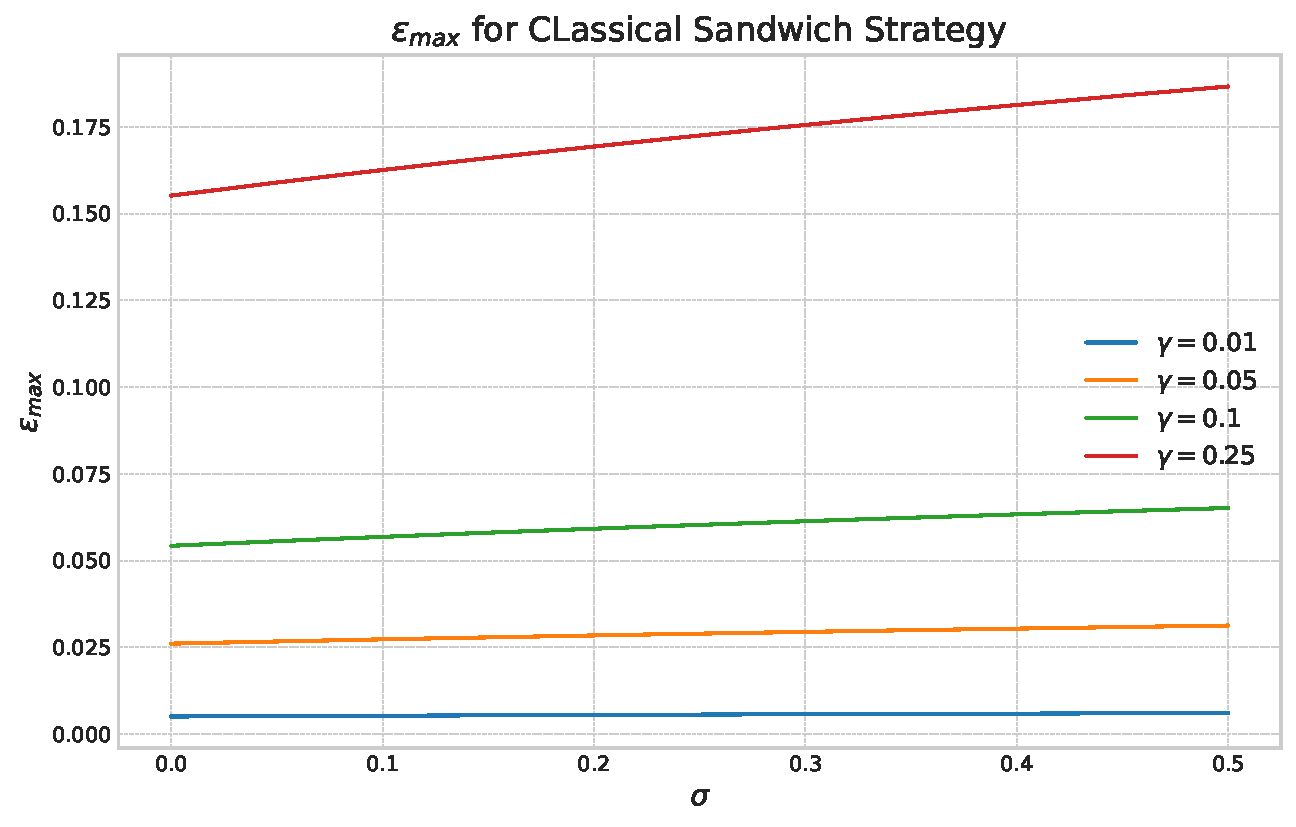
\includegraphics[width=0.7\linewidth]{figures_st_app/epsilon_max_sand.pdf}
    \caption{Caption}
    \label{fig:eps_max}
\end{figure}

%---------------------------------------------------------------------------
\paragraph{Back-run swap (Y$\to$X).} Finally, $\Delta y_{\mathrm{fr}}$ are traded back in the back-run swap from $Y$ to $X$. The amount that the searcher gets back is

\begin{equation}
\Delta x_{\text{br}} = x_0\frac{r^2 \varepsilon (1 + r\varepsilon + r\sigma)^2}{(1 + r\varepsilon) + r^2 \varepsilon (1 + r\varepsilon + r\sigma)}.
\end{equation}


%---------------------------------------------------------------------------
Not considering for the moment gas and bribe costs, the searcher's profit is the difference between the input amount in the front-run swap and the output amount in the back-run swap

\begin{equation}
\Pi_{sand}(\varepsilon, \sigma) = \Delta x_{\text{br}} - s = x_0 \left[\frac{r^2 \varepsilon(1 + r\varepsilon + r\sigma)^2}{(1 + r\varepsilon) + r^2 \varepsilon (1 + r\varepsilon + r\sigma)} - \varepsilon \right]
,
\label{eq:Pi_exact}
\end{equation}

\begin{equation}
\pi_{sand}(\varepsilon, \sigma) = \frac{\Pi}{x_0}
\label{eq:pi_exact}
\end{equation}

We can obtain the value of $\sigma$ that turn on the profits:

\begin{equation}
    \pi_{sand}(\varepsilon, \sigma) >0 \quad \text{when} \quad \sigma>\sigma_{min} = \frac{1}{r}\left(\frac{\varepsilon+\sqrt{\varepsilon^2 + \frac{4(1+r\varepsilon)}{r^2}}}{2}-1 - r\varepsilon \right) \underset{\varepsilon\to0^+}\approx f
\end{equation}
%---------------------------------------------------------------------------
Now we want to obtain the optimal value to trade in the front-run swap that maximizes the profit. In other words, we want to solve the following problem
\begin{align}
    \text{maximize } & \  \pi_{sand}(\varepsilon, \sigma) \nonumber\\ 
    \text{subject to } & \varepsilon \leq \varepsilon_{\text{max}}(\sigma, \gamma, r)
\end{align}
The first-order condition leads to a quartic equation whose solution can be found numerically. 

The constraint given by the slippage requires that the actual maximum $\varepsilon^*$ be
\begin{equation}
    \varepsilon^* = \min{\{\varepsilon_+, \varepsilon_{\text{max}}(\sigma, \gamma, r)\}}
\end{equation}
If we substitute this value in the profit expression, we get
\begin{equation}
    \pi_{sand}^*(\varepsilon,\sigma) = \frac{r^2 \varepsilon^* (1 + r\varepsilon^* + r\sigma)^2}{(1 + r\varepsilon^*) + r^2 \varepsilon^* (1 + r\varepsilon^* + r\sigma)} - \varepsilon^*
\end{equation}

%---------------------------------------------------------------------------
%  3.3  Sandwich attack option — size-based dominance
%---------------------------------------------------------------------------

Define the gas spread and the gas spread per reserve.
\begin{equation}
\delta' := G_{\text{JIT}}-G_{\text{sand}},\qquad
\phi'   := \frac{\delta'}{x_{0}}\quad
\end{equation}
The two bribe ceilings are

\[
\begin{aligned}
m_{\max}^{\text{JIT}} 
   &= S f - G_{\text{JIT}} 
   = x_{0} \bigl(\sigma f - \phi' \bigr), \\
m_{\max}^{\text{sand}} 
   &= x_{0} \pi^*.
\end{aligned}
\]

The builder includes the JIT bundle when its
bribe ceiling exceeds the sandwich one:

\begin{equation}
x_{0}\,\bigl(\sigma f - \phi'\bigr)
   \;\ge\;
x_{0}\,\pi^*
\quad\Longleftrightarrow\quad
F(\sigma)\;:=\;
\sigma f - \phi' - \pi^*\;\ge 0.
\end{equation}

Because \(F(0)=-\phi' < 0\) (if JIT has any gas handicap)
and \(F(\sigma)\to \infty\) as \(\sigma\to\infty\),
there is (under regular fee-tier ranges) a unique positive root
\(\sigma_{\text{sand}}^{\ast}\) that solves \(F(\sigma)=0\). Therefore, we have that the JIT strategy wins against the sandwich attack alternative when

\begin{equation}
\boxed{%
   \sigma \;\ge\; \sigma_{\text{sand}}^{\ast}(f,\phi')
}
\qquad\Longleftrightarrow\qquad
\boxed{%
   S      \;\ge\; S_{\text{sand}}^{\ast}:=
            \sigma_{\text{sand}}^{\ast}\,x_{0}
}.
\end{equation}

Figure \ref{fig:frontrun_size_vs_profit} represents the relationship between the front-run size $\varepsilon$ and the sandwich profit $\pi(\varepsilon)$. As we can see, the profit reaches a maximum and then starts to decreases afterward. The decreasing can also lead to negative profits, especially for low liquidity pools. However, the maximum is never actually reached by the searcher. Also in this case, the slippage tolerance does not let the attacker to extract the most of the rent.

\subsection{Mixed (Sandwich + JIT) attack}
\label{subsec:mixed-sandwich-jit}

We analyze a bundle that combines a self-funded sandwich with JIT liquidity provision. The sequence consists of a front-run swap, a front-run mint, a set of victim swaps, a back-run burn, and a back-run swap. The goal is to profit both from the sandwich’s price impact and the JIT fee capture. Because the JIT deepens the book during the victim leg, the victim’s min-out constraint is easier to satisfy, which allows a larger feasible front-run size~$\varepsilon$. To the best of out knowledge, there is currently no study in the literature that accounts for this strategy. Furthermore, we were not able to find any particular information even on the web, even if data clearly shows the occurrence of this pattern, as highlighted in \cite{gatta_di_nosse}

\paragraph{Front-run swap (X$\to$Y).}
The attacker swaps $s=\varepsilon x_0$ (user input), so the effective input is $r s$. With constant product and fee on input,
\begin{equation}
  \Delta y_{\mathrm{fr}} \;=\; y_0\,\frac{r\varepsilon}{1+r\varepsilon},
  \qquad
  (x_0,y_0)\mapsto (x_1,y_1)=\bigl(x_0(1+r\varepsilon),\, y_0/(1+r\varepsilon)\bigr).
  \label{eq:mix_dyfr}
\end{equation}

\paragraph{Front-run JIT mint.}
To avoid changing price, it is convenient to parametrize the added reserves with respect to the current ones. If $\alpha$ of the \emph{post-FR} reserves is added, the state scales as
\begin{equation}
  (x_1,y_1) \;\mapsto\; (x_2,y_2) \;=\; \bigl(x_1(1+\alpha),\, y_1(1+\alpha)\bigr)
  \;=\; \Bigl(x_0(1+r\varepsilon)(1+\alpha),\, \frac{y_0(1+\alpha)}{1+r\varepsilon}\Bigr).
  \label{eq:mix_mint}
\end{equation}
Therefore the attacker owns a a fraction $\frac{\alpha}{\alpha + 1}$ of the active range.

\paragraph{Victim swap(s) (X$\to$Y).}
Size $S=\sigma x_0$; effective input $rS$. From \eqref{eq:mix_mint}, the victim’s Y out is
\begin{equation}
  \Delta y_v
  \;=\; \left(\frac{y_0}{1+r\varepsilon}\right)\!\cdot
         \frac{(1+\alpha)\,r\sigma}{(1+r\varepsilon)(1+\alpha)+r\sigma},
  \label{eq:mix_dyv}
\end{equation}
and the state becomes (still with JIT present)
\begin{equation}
  (x_3,y_3) \;=\;
  \Bigl(x_0\bigl((1+r\varepsilon)(1+\alpha)+r\sigma\bigr),\;
        \frac{y_0(1+\alpha)^2}{(1+r\varepsilon)(1+\alpha)+r\sigma}\Bigr).
  \label{eq:mix_state_with_jit_after_victim}
\end{equation}
Slippage feasibility is the same as in §3.3 but in this case the enhanced liquidity allows for a bigger $\varepsilon_{\text{max}}$ (see Figure \ref{fig:eps_max_jit_sand}):
\begin{equation}
  \Delta y_v \;\ge\; (1-\gamma)\,\Delta y_{\mathrm{base}},
  \quad \Delta y_{\mathrm{base}}=y_0\,\frac{r\sigma}{1+r\sigma},
  \quad\Longrightarrow\quad
  \varepsilon \le \varepsilon_{\max}(\sigma,\gamma,r, \alpha).
  \label{eq:mix_eps_cap}
\end{equation}
where

\begin{equation}
    \varepsilon_{\max}(\sigma,\gamma,r, \alpha) = \frac{1}{r}\left[\frac{-r\sigma + \sqrt{(r\sigma)^2+ \frac{4(1+\alpha)^2(1+r\sigma)}{1-\gamma}}}{2(1+\alpha)}-1 \right]
\end{equation}

\begin{figure}
    \centering
    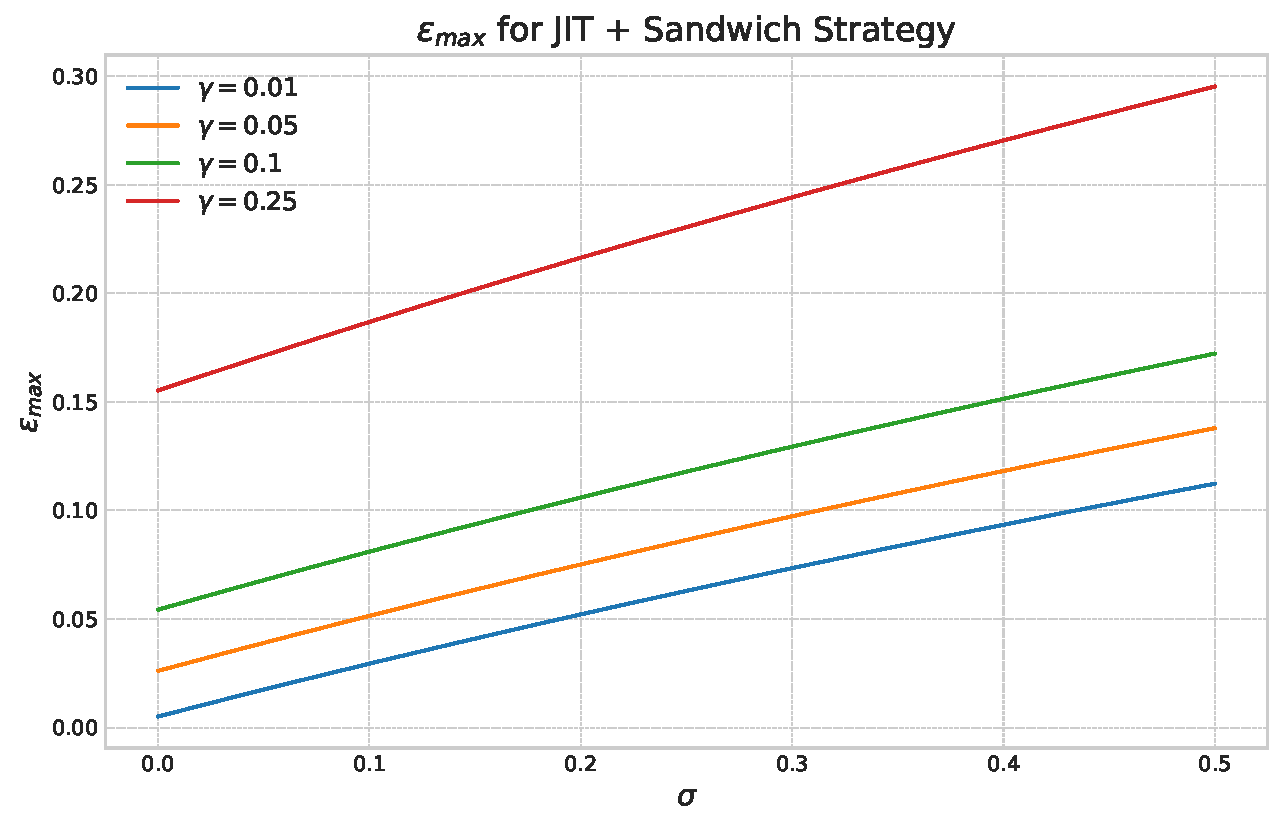
\includegraphics[width=0.7\linewidth]{figures_st_app/epsilon_max_jit_sand.pdf}
    \caption{Maximum normalized front run amount $\epsilon_{max}$ vs normalized victim's swap amount $\sigma$ for different values of the slippage tolerance $\gamma$. The value of $\alpha$ is set to 1 (i.e. LP owns half of the active tick range).}
    \label{fig:eps_max_jit_sand}
\end{figure}

\paragraph{Back-run burn (JIT).}
Immediately after the victim, the JIT LP is burned. Since the position was proportional, burning removes a fraction $\alpha/(1+\alpha)$ of both reserves, so the base-pool state is
\begin{equation}
  (x_4,y_4) \;=\; \frac{1}{1+\alpha}\,(x_3,y_3)
 \;=\; \Bigl(x_0\bigl((1+r\varepsilon)+\frac{r\sigma}{1+\alpha}\bigr),\;
             \frac{y_0(1+\alpha)}{(1+r\varepsilon)(1+\alpha)+r\sigma}\Bigr).
  \label{eq:mix_state_after_burn}
\end{equation}
After the burn, the attacker ends up with 
\begin{equation}
    \Delta x_{burn} = \frac{\alpha}{\alpha + 1} x_3 = \frac{x_0\alpha}{\alpha + 1}
\end{equation}
$\alpha x_0(1+r\varepsilon) + \frac{\alpha}{\alpha +1}r \sigma x_0$ tokens X and $\alpha y_0 - \frac{\alpha}{\alpha +1}\Delta y_v$ of tokens Y.

\paragraph{Back-run swap (Y$\to$X).}
The attacker now has to swap in the opposite direction than victims' swaps. 

\begin{equation}
    x_4 y_4 = \bigl( x_4 - \Delta x_{br}\bigr)\bigl(y_4 + r\Delta y_{br}\bigr)
\end{equation}

We can derive the expression of $\Delta x_{br}$ with respect to $x_0$. Let $\theta = \frac{\Delta y_{br}}{y_0}$

\begin{equation}
\Delta x_{br} = x_0 \left\{\frac{\left[(1+r\varepsilon)(1+\alpha) + r\sigma\right]^2r\theta}{(1+\alpha)\left[(1+\alpha) + \left((1+\alpha)(1+r\varepsilon)+r\sigma\right)r\theta\right]} \right\}
\end{equation}

\paragraph{Profit.} The profit the attacker obtains is composed of the difference between the back-run output amount and the front-run input amount (the same as in the case of the classical sandwich) plus the fees collected by the LP position plus the difference between the tokens' amounts burnt and minted

\begin{equation}
    \Pi_{sand+jit}(\varepsilon,\sigma, \alpha) = \underbrace{\bigl(\Delta x_{br} - \varepsilon x_0 \bigr)}_{\text{Sandwich}} + \underbrace{\sigma x_0f\frac{\alpha}{\alpha + 1}}_{\text{LP fees}} + \underbrace{x_0\alpha r \sigma \left[\frac{1}{1+\alpha}-\frac{1}{(1+r\varepsilon) \left( (1+\alpha)(1+r\varepsilon)+r\sigma\right)}\right]}_{\text{LP inventory}}
\end{equation}

Therefore, normalizing the profit with respect to $x_0$ and substituting the full expression for $\Delta x_{br}$, we obtain
\begin{equation}
\begin{aligned}
\pi_{sand+jit}(\varepsilon, \alpha, \sigma) 
= &\left\{ \frac{\left[(1+r\varepsilon)(1+\alpha) + r\sigma\right]^2 r\theta}
{(1+\alpha)\left[(1+\alpha) + \left((1+\alpha)(1+r\varepsilon)+r\sigma\right)r\theta\right]} - \varepsilon \right\} \\
&+ \frac{\sigma f \alpha}{\alpha + 1} 
+ \alpha r \sigma \left[ \frac{1}{1+\alpha} - \frac{1}{(1+r\varepsilon)\left((1+\alpha)(1+r\varepsilon)+r\sigma\right)} \right]
\end{aligned}
\end{equation}


In general, we have two options for $\theta y_0$
: (i) keep the self funding framework as in the classical sandwich attack or (ii) let the back run amount to be a new free parameter. Currently we did not study the second option since empirically we almost always find the self funded option, as we can see from Figure \ref{fig:obs_vs_pred_backrun}.

\begin{figure}
    \centering
    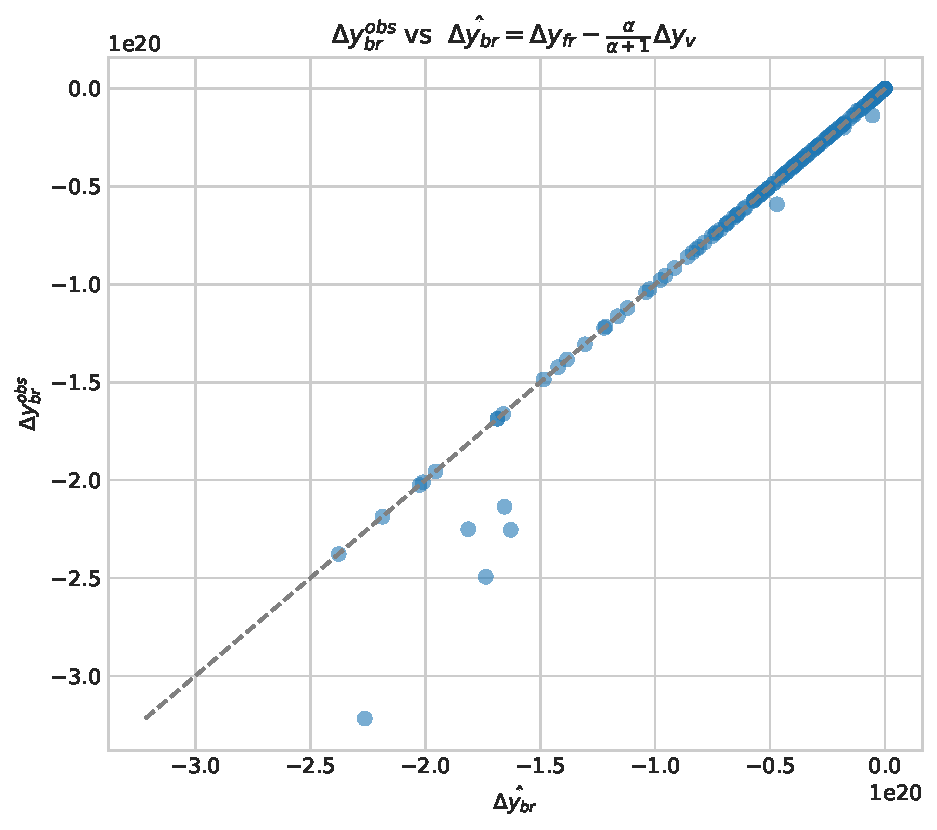
\includegraphics[width=0.5\linewidth]{figures_st_app/obs_vs_pred_backrun.pdf}
    \caption{Relation between the back run swap amount observed on-chain $\Delta y_{br}^{obs}$ and the theoretical one $\Delta y_{br}$ based on the self funding condition.}
    \label{fig:obs_vs_pred_backrun}
\end{figure}

Differently from the case of the self funded sandwich attack, in this case the back run amount is not equal to the front run amount, because the LP position has already hedged part of the attacker exposure obtained after the front run. Specifically, during the victims' swap, the attacker takes the opposite side of the trades, giving $\frac{\alpha}{ (1+\alpha)}\Delta y_v$ tokens $Y$ and receiving $\frac{\alpha}{ (1+\alpha)}rS$ of tokens X. Therefore, she has only to back run the residual $\theta_{self} = \frac{1}{y_0}\left(\Delta y_{fr} - \frac{\alpha}{1+\alpha} \Delta y_v\right)$. Empirically it is actually what we see.

In this case, the LP inventory change in tokens Y is fed as a minus component into the back run amount. The profit is therefore 

\begin{equation}
    \Pi_{sand+jit}(\varepsilon, \alpha, \sigma) = \underbrace{\bigl(\theta_{self}y_0 - \varepsilon x_0 \bigr)}_{\text{Sandwich Profit}} + \underbrace{\frac{\alpha\sigma x_0f}{\alpha + 1}}_{\text{LP fees}} + \underbrace{ \frac{x_0\alpha r \sigma}{\alpha+1}}_{\text{LP inventory change in X}}
\end{equation}

The full expression is

\begin{equation}
\pi_{sand+jit}(\varepsilon, \alpha, \sigma) = \frac{[(1 + r\varepsilon)(1 + \alpha) + r\sigma ]^2r\theta_{self}}{(1 + \alpha)\left[(1 + \alpha) + ((1 + \alpha)(1 + r\varepsilon) + r\sigma) r\theta_{self}\right]} - \varepsilon + \frac{\alpha\sigma}{\alpha + 1}
\end{equation}

where
\begin{equation}
    \theta_{self} = \frac{r}{1+r\varepsilon} \left[\varepsilon - \frac{\alpha \sigma}{(1+r\varepsilon)(1+\alpha)+r\sigma}\right]
\end{equation}

When $\theta_{self}\leq0$ the (normalized) fees earned by the LP is bigger that $\epsilon$, flipping the sign of the back run swap. Therefore, to not incur in a loss, the MEV searcher chooses to perform a pure JIT.

The maximization problem is 

\begin{equation}
\begin{aligned}
\max_{\varepsilon,\alpha} \;\; \pi_{\text{sand+jit}} \quad \text{subject to} \quad
\begin{cases}
0 \leq \varepsilon \leq \varepsilon_{\max} \\
\alpha \geq 0 \\
\theta_{self} >0
\end{cases}
\end{aligned}
\end{equation}

The results have been obtained numerically searching for $\varepsilon^* \in [\varepsilon_{min}, \infty]$ and $\alpha \in [0, \alpha_{max}]$ with $\varepsilon_{min}=10^{-9}$ and $\alpha_{max} = 1$. Actually, the optimizer always pushes $\alpha^* \to \alpha_{max}$, whatever its value is. Figure \ref{fig:regime_transition} shows  $\varepsilon^*$ and $\alpha^*$ as a function of the normalized victim's input size $\sigma$ for $f=0.01\%, 0.05\%, 0.3\%$. Except in the case of the $0.01\%$, we can see that there is a quite sharp transition between two different regimes:

\begin{enumerate}
    \item Pure JIT, where $\varepsilon$ is pushed to $\varepsilon_{min}$ and $\alpha$ to $\alpha_{max}$
    \item Combination of JIT and Sandwich attack with 
\end{enumerate}

\begin{figure}
    \centering
    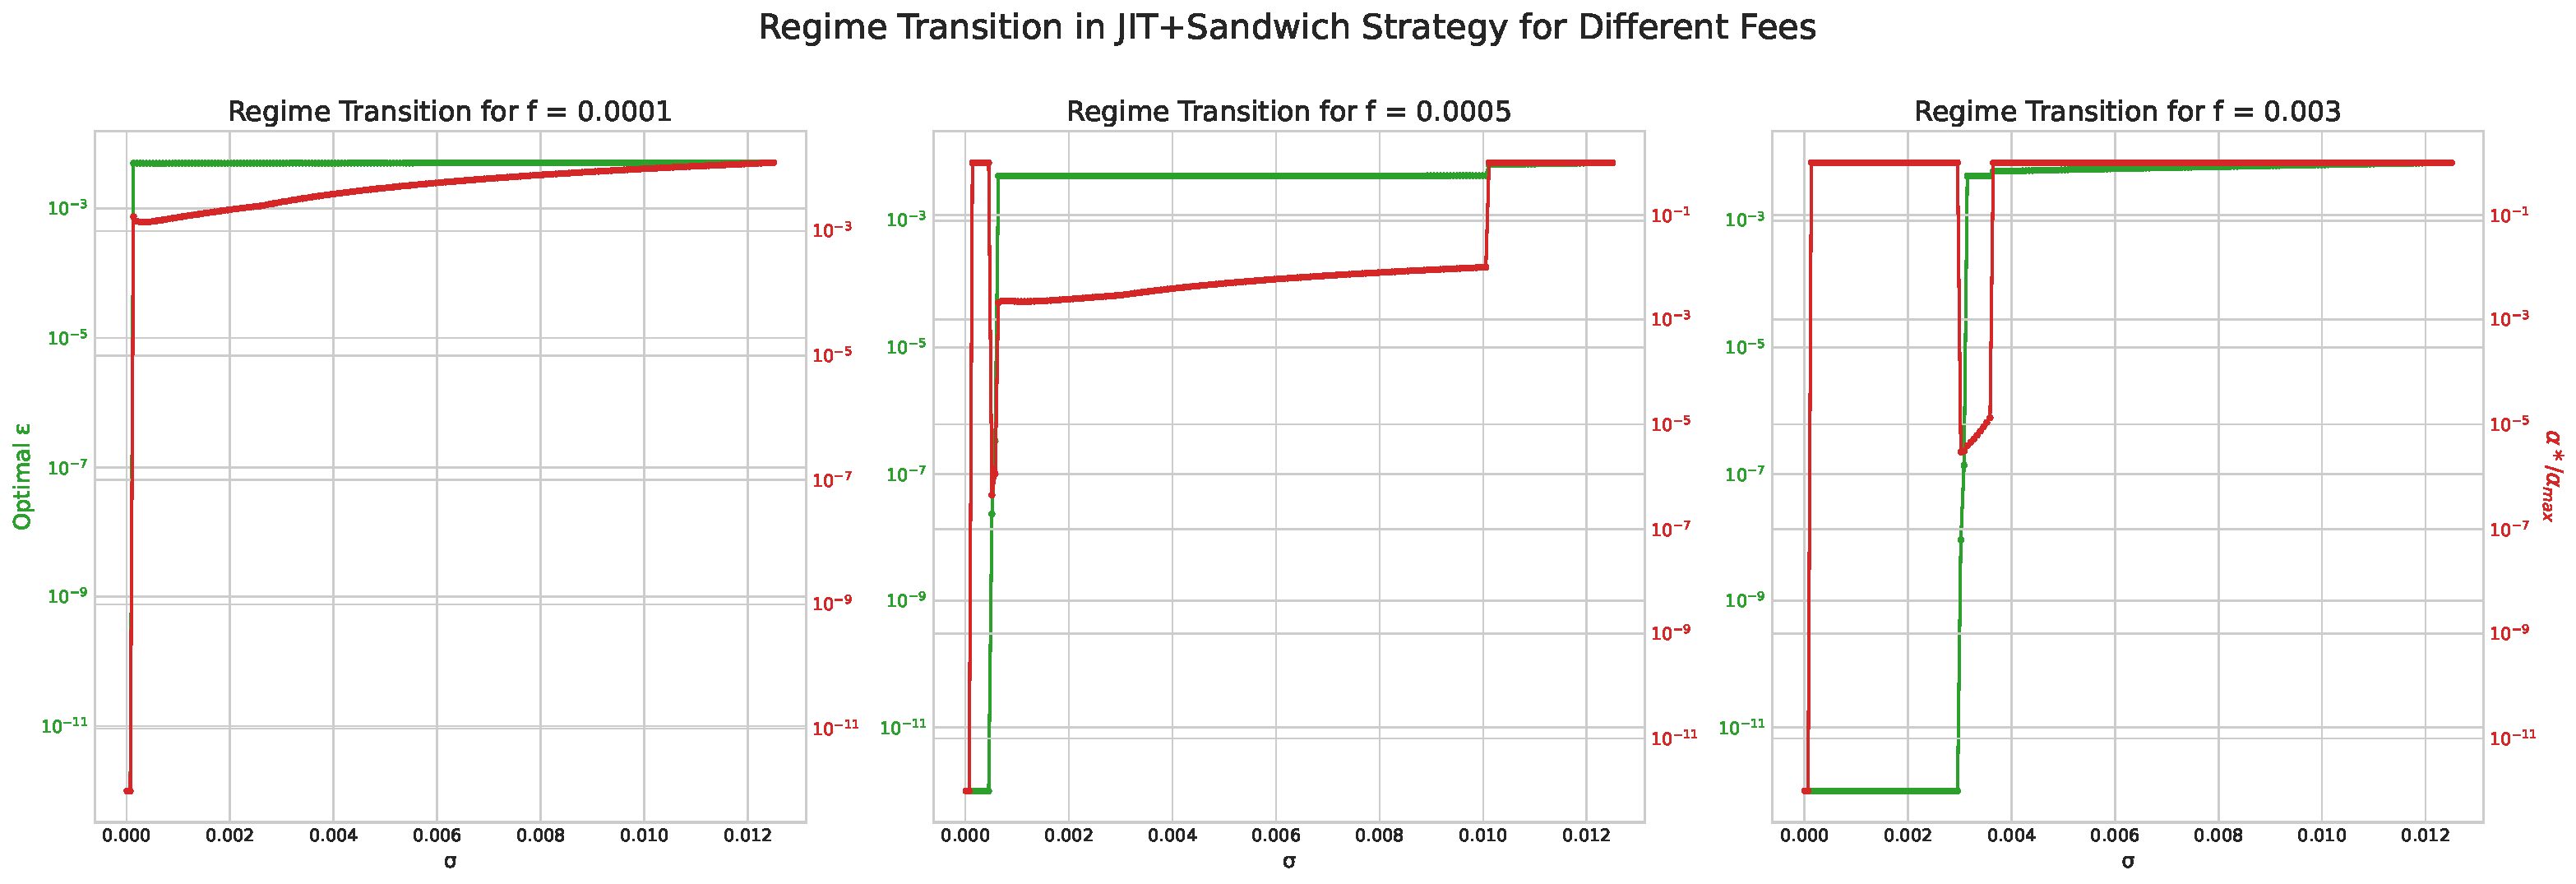
\includegraphics[width=1\linewidth]{figures_st_app/regime_transition_subplots.pdf}   \caption{Optimal values for $\varepsilon$ and $\alpha$ with respect to $\sigma$ for different values of the fee tier.}
    \label{fig:regime_transition}
\end{figure}

Figure \ref{fig:profits_comparison} shows the dynamics of the four ceilings (profits) for the three MEV strategies discussed so far for different fee tiers. One can be surprised by the fact that a classic sandwich attack is less profitable than an arbitrage trade after a certain value of $\sigma$. This is due to how we treated the sandwich attack strategy. Indeed, we set up a self funded strategy, in which the back run amount is equal to the front run size. Due to the presence of the slippage tolerance, the maximum front-run size $\varepsilon_{max}$ is limited. Therefore, also the maximum profit achievable will be affected by this constraint. On the other hand, we do not have any limit on the arbitrage back-run that depends only on the victim swapped size $\sigma$. Anyway, combining a classical sandwich with a JIT, allows for a greater front run size and a flow of fee towards the searcher. This makes the mixed strategy the most profitable one for $f=0.3\%$. For lower ones, the difference between the classical sandwich and the mixed strategy becomes negligible. As we can see from the graphs, the transition between a pure JIT and a mixed strategy happens at $\sigma=f$.


\begin{figure}
    \centering
     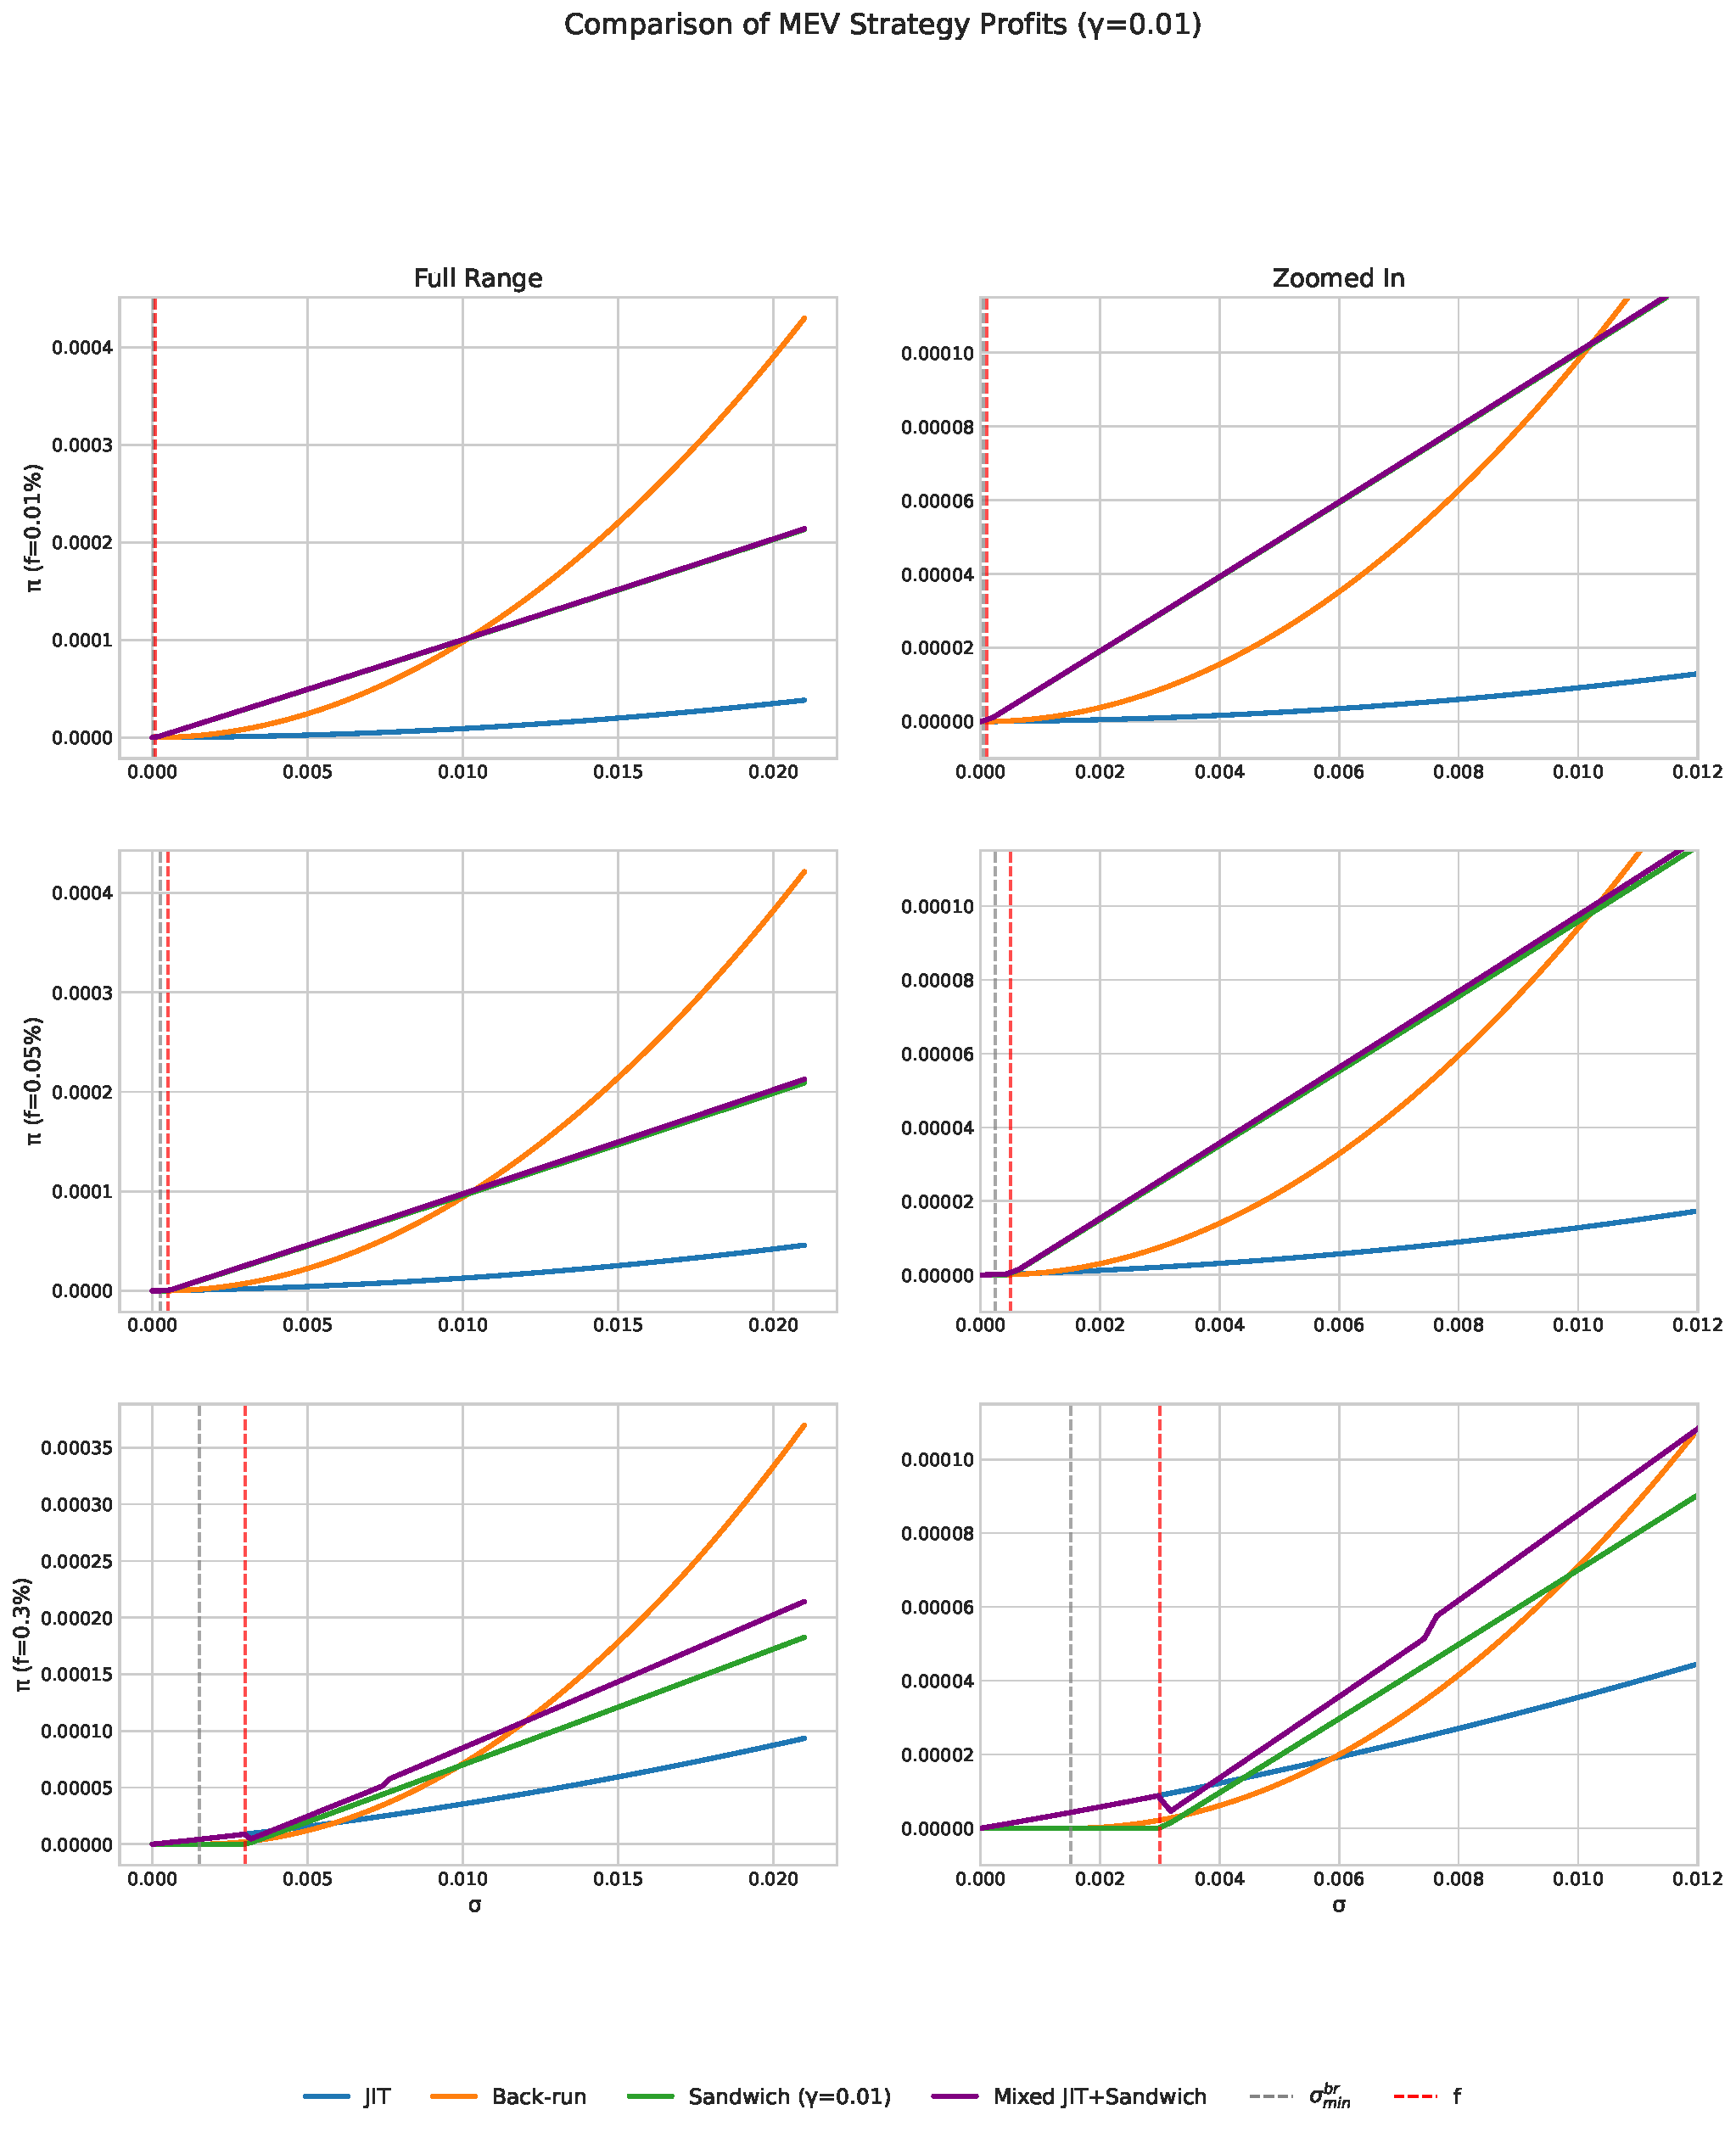
\includegraphics[width=0.9\linewidth]{figures_st_app/profits_comparison.pdf}
    \label{fig:profits_comparison}
    \caption{Visualization of the profits of the different MEV strategies for $f\in[0.01\%,0.05\%,0.3\%]$ and slippage $\gamma=1\%$. The vertical gray dashed line corresponds to the minimum value of $\sigma$ that induces a price change greater than the fee tier, while the red dashed line highlights the pool's fee rate. The gas fees are set to zero.}
\end{figure}

\begin{figure}
    \centering
    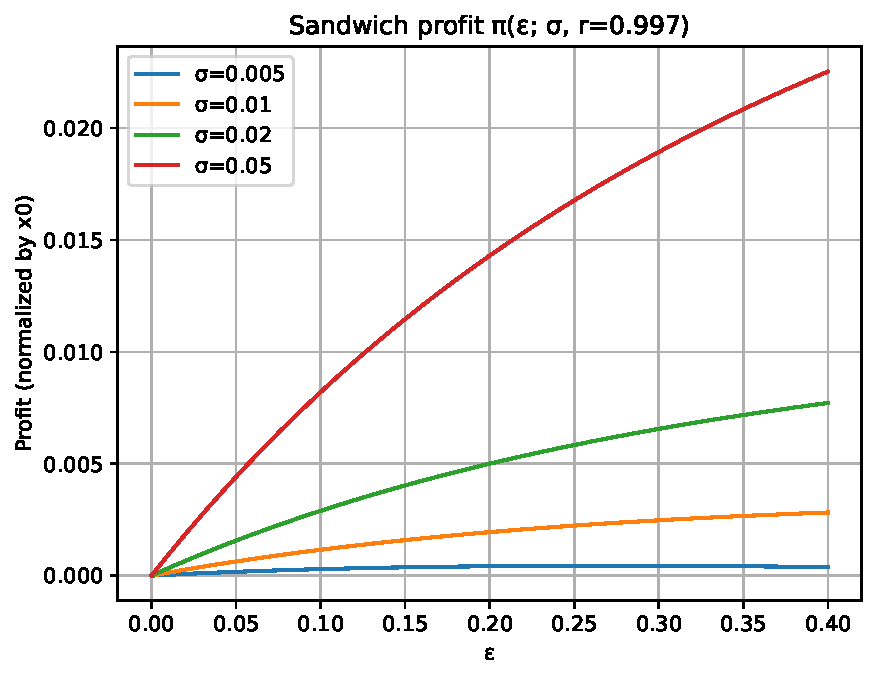
\includegraphics[width=0.7\linewidth]{figures_st_app/sandwich_profit_vs_epsilon.pdf}
    \caption{Sandwich profits vs $\varepsilon$. The vertical dashed lines correspond to th e maximum value of the front run size $\varepsilon_{max}(\gamma)$ for different value of the slippage tolerance $\gamma$. Fee tier 0.05\%, $x_0=1$.}
    \label{fig:frontrun_size_vs_profit}
\end{figure}

\section{Empirical profits}
Currently I have collected MEV patterns discussed in the previous sections for the 2023 and for the USDC-WETH 0.05\% pool. The goal is to check the validity of the relationship obtained in the previous section regarding the MEV strategy profits.

The heuristic used to collect the arbitrage swaps is inherently noisy: a swap that changed the price for a quantity greater than the fee tier is not necessarily followed by an arbitrage swap. In other words, even if there is a swap in the opposite direction, it can be a coincidence. Therefore, I applied a stronger heuristic, collecting only the swaps that pushed the price back to $1\%$ of the target $rP_0$.

Profits are evaluated based on actual on-chain data as the difference between what the searcher paid and what was obtained from the strategy. There is therefore no bias due to the theory discussed above, except for the condition imposed while collecting back run arbitrages.

Finally, no gas costs have been considered.

The JIT and classical sandwich attacks profits seem to follow the behavior obtained in the theoretical sections. However, for sandwich profits we found
\begin{itemize}
    \item A lot of negative profits. Almost all of them are related to $\sigma < \sigma_{min}$
    \item A lot of back run arbitrages with almost zero profits
\end{itemize}

As shown in Figure \ref{fig:empirical_profits} , there are some discrepancies between theory and empirical evidences. For instance, the onset of positive profits for both the sandwich attacks/mixed strategy and the back run arbitrages happens for $\sigma$ values a bit greater than the predicted ones. Possible sources of this discrepancy can be (i) not optimality in strategy settings or, more probably, (ii) cross-tick effects that we did not account for

\begin{figure}
    \centering
    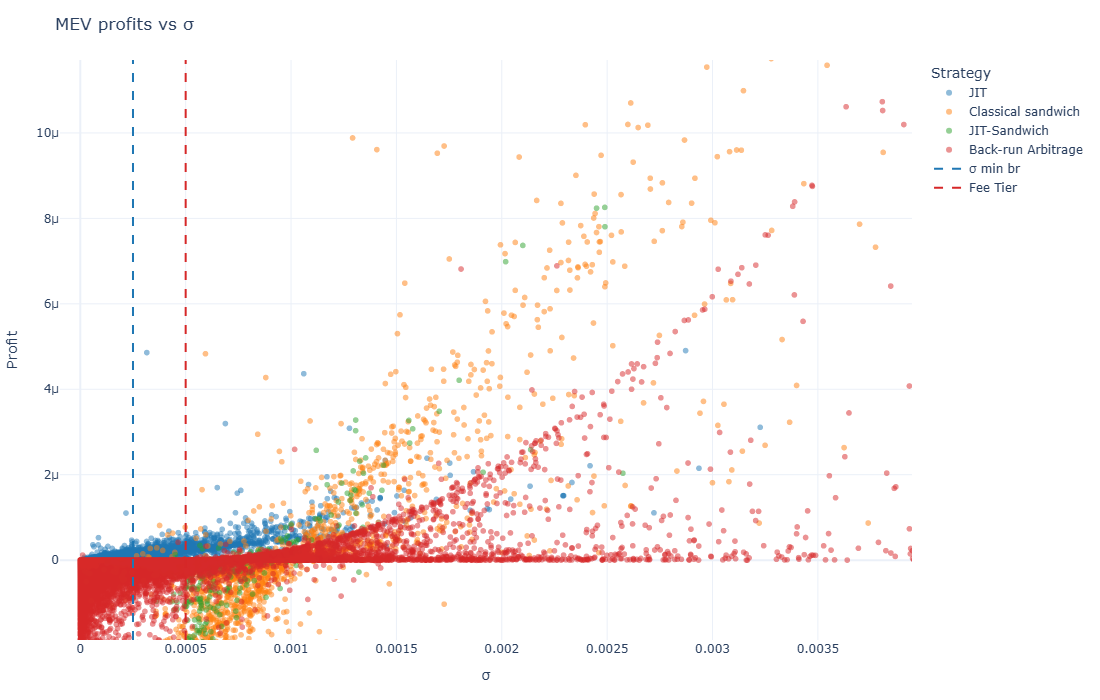
\includegraphics[width=0.7\linewidth]{figures_st_app/empirical_profits.png}
    \caption{Caption}
    \label{fig:empirical_profits}
\end{figure}

\appendix
\section{Tick-aware rules for Uniswap v3 execution}
\label{app:tick-rules}

\paragraph{State and notation.}
Let \(S=\sqrt{P}\) denote the square-root price (X in Y) and \(L\) the \emph{active} liquidity of the current tick whose boundaries are \((S_\ell,S_u)\) with \(S_\ell<S<S_u\).
The pool charges a fee-on-input \(f\); write \(r=1-f\).
For intuition within a tick, define the virtual reserves \(\tilde x=L/S\) and \(\tilde y=L\,S\) (so \(\tilde x\,\tilde y=L^2\)).
Only \emph{swaps} move price; \emph{mints/burns} are price-neutral.

\subsection{Swaps within a tick (price update and amounts)}
\label{app:swaps-within-tick}
\textbf{X\(\to\)Y (consume X, output Y).}
For effective input \(x_{\mathrm{eff}}=r\,x_{\mathrm{in}}\):
\begin{equation}
S'=\frac{1}{\,S^{-1}+x_{\mathrm{eff}}/L\,},\qquad
\Delta y = L\,(S'-S),\qquad
\text{fees in X} = f\,x_{\mathrm{in}}.
\end{equation}

\noindent
\textbf{Y\(\to\)X (consume Y, output X).}
For effective input \(y_{\mathrm{eff}}=r\,y_{\mathrm{in}}\):
\begin{equation}
S' = S + \frac{y_{\mathrm{eff}}}{L},\qquad
\Delta x = L\Big(S^{-1}-S'^{-1}\Big),\qquad
\text{fees in Y} = f\,y_{\mathrm{in}}.
\end{equation}

\noindent\emph{Interpretation.}
Within a tick these are exactly the constant-product updates on \((\tilde x,\tilde y)\) using the \emph{effective} input \(r\) (fees are withheld from input and added to the pool in the input token).
Signs \(\Delta x,\Delta y\) above are pool-side deltas (amounts received by the trader have opposite sign).

\subsection{Tick boundaries (capacity and traversal)}
\label{app:boundaries}
\textbf{Capacity to the lower boundary} \(S_\ell\) for a \emph{downward} move (X\(\to\)Y):
\begin{equation}
x_{\max}^{(\mathrm{eff})}=L\!\left(\frac{1}{S_\ell}-\frac{1}{S}\right),\qquad
x_{\max}= \frac{x_{\max}^{(\mathrm{eff})}}{r}.
\end{equation}

\noindent
\textbf{Capacity to the upper boundary} \(S_u\) for an \emph{upward} move (Y\(\to\)X):
\begin{equation}
y_{\max}^{(\mathrm{eff})}=L\,(S_u-S),\qquad
y_{\max}=\frac{y_{\max}^{(\mathrm{eff})}}{r}.
\end{equation}

\noindent
\textbf{Boundary rule.}
When a boundary is reached, update the active liquidity
\begin{equation}
L \leftarrow L \pm \Delta L_{\mathrm{tick}},
\end{equation}
where \(\Delta L_{\mathrm{tick}}\) is the net liquidity change encoded at that boundary; then advance to the next active tick \((S_\ell,S_u)\) and continue.
(Only the \emph{active} tick’s \(L\) affects price moves.)

\subsection{Liquidity changes (mints and burns)}
\label{app:mints-burns}
\paragraph{General mint (range \([\;S_a,S_b\;]\) with \(S_a<S_b\)).}
Adding \(\Delta L\) does \emph{not} move price.
The deposited principal amounts at current \(S\) are
\begin{equation}
(\Delta x,\Delta y)=
\begin{cases}
\Big(\Delta L\!\big(\dfrac{1}{S_a}-\dfrac{1}{S_b}\big),\; 0\Big), & S\le S_a,\\[8pt]
\Big(\Delta L\!\big(\dfrac{1}{S}-\dfrac{1}{S_b}\big),\; \Delta L\,(S-S_a)\Big), & S_a<S<S_b,\\[8pt]
\Big(0,\; \Delta L\,(S_b-S_a)\Big), & S\ge S_b.
\end{cases}
\end{equation}
If \(S\in[S_a,S_b)\), the position is \emph{active} and the active liquidity becomes \(L\leftarrow L+\Delta L\).
If \(S\notin[S_a,S_b)\), the deposit is \emph{inactive now} (no change to active \(L\)) and becomes active only when price re-enters the range.

\paragraph{JIT mint (ultra-narrow around the current tick).}
Take \([S_a,S_b]\) to coincide with the current tick; set \(\alpha=\Delta L/L_{\mathrm{base}}\).
Then, while price stays in the tick,
\begin{equation}
L \leftarrow (1+\alpha)\,L_{\mathrm{base}},\qquad
(\tilde x,\tilde y)\ \text{scale by }(1+\alpha).
\end{equation}
This is the formal justification for the “state scales by \(1+\alpha\)” step used in Section~3.
If price leaves the tick before a burn, the JIT position becomes \emph{inactive} (it no longer contributes to active \(L\)) until price re-enters or the position is burned.

\paragraph{General burn (range \([\;S_a,S_b\;]\)).}
Removing \(\Delta L\) does \emph{not} move price.
The withdrawn principal at current \(S\) is
\begin{equation}
(\Delta x,\Delta y)=
\begin{cases}
\Big(\Delta L\!\big(\dfrac{1}{S_a}-\dfrac{1}{S_b}\big),\; 0\Big), & S\le S_a,\\[8pt]
\Big(\Delta L\!\big(\dfrac{1}{S}-\dfrac{1}{S_b}\big),\; \Delta L\,(S-S_a)\Big), & S_a<S<S_b,\\[8pt]
\Big(0,\; \Delta L\,(S_b-S_a)\Big), & S\ge S_b.
\end{cases}
\end{equation}
If the position is \emph{active} at burn time, update active liquidity \(L\leftarrow L-\Delta L\).
If the position is \emph{inactive}, burning does not change active \(L\) (you still withdraw principal computed at current \(S\) per the cases above).

\paragraph{Fee accruals for mints/burns.}
Fees are collected \emph{pro-rata to active liquidity and only while the position is active}.
In a swap that consumes input \(q\) with fee \(f\), the pool retains \(f\,q\) of the \emph{input} token; a position active during that swap accrues the share
\(\dfrac{\Delta L}{L_{\mathrm{active}}}\times f\,q\)
(up to rounding) into its uncollected fees.
Burning (or an explicit \texttt{collect}) realizes the position’s uncollected fees in their respective tokens \emph{in addition to} the principal amounts above.
For a JIT mint active only for the victim swap, the fee share during that swap is \(\dfrac{\alpha}{1+\alpha}\) of the victim’s fee in the input token (again subject to rounding and any protocol fee).

\end{document}